\documentclass[letterpaper,12pt]{article}

\usepackage[utf8]{inputenc} % Para asegurar compatibilidad en Windows y GNU/Linux
\usepackage[spanish]{babel} % Idioma de entrada
\spanishdecimal{.} % Cambia en las ecuaciones el símbolo separador de decimales. Por defecto se
% usa coma "," pero en español se utiliza punto "."1
\usepackage[right=2cm,left=2.5cm,top=2.5cm,bottom=2.8cm,headsep=1cm,footskip=1.5cm]{geometry} % Márgenes conforme a lo requerido en el reglamento de pregrado.
\usepackage{fancyhdr}% Cabeceras y pie de página en páginas internas
\pagestyle{fancy} % Definición del encabezado
\lhead{Informe avance Proyecto HP.} 
\rhead{Felipe A. Seguel Mora} 
\cfoot{\thepage}
\usepackage{graphicx,tabularx,latexsym} % Para insertar gráficos, figuras y tablas
\usepackage{subfigure}
\usepackage{amsmath}
\usepackage{appendix}

%\usepackage{acronym}

\usepackage{listings}
% Matemáticas avanzadas
\usepackage{amsthm,amsmath,amssymb,amsfonts}
\usepackage[anchorcolor=black,% Crea pdf con hipervínculos. Cambiar colorlinks y/o blue a black para eliminar los colores 
            citecolor=blue,
	    	colorlinks=true,
            filecolor=blue,
            letterpaper,
            bookmarksnumbered=true,
            bookmarksopen=true,
            linktocpage,
            linkcolor=blue,
            menucolor=blue,
            pagecolor=blue,
            urlcolor=blue,]{hyperref}
\usepackage{bm}% Para legras griegas en negrita.
\usepackage{titlesec}

\setcounter{secnumdepth}{4}

\titleformat{\paragraph}
{\normalfont\normalsize\bfseries}{\theparagraph}{1em}{}
\titlespacing*{\paragraph}
{0pt}{3.25ex plus 1ex minus .2ex}{1.5ex plus .2ex}

% Para tener subfiguras
% Ref: http://www.fi.infn.it/pub/tex/doc/orig/subfigure.pdf
\usepackage{subfigure}
\usepackage{float}
\newcommand{\compresslist}{ % Define a command to reduce spacing within itemize/enumerate environments, this is used right after \begin{itemize} or \begin{enumerate}
\setlength{\itemsep}{1pt}
\setlength{\parskip}{0pt}
\setlength{\parsep}{0pt}
}
\clubpenalty=10000 % Penalizar lineas huérfanas.
\widowpenalty=10000 % Penalizar líneas viudas.

\begin{document}

% ***********************************************************************************
\renewcommand{\contentsname}{Índice general.}% Redefinir nombres conforme reglamento de pregrado.
\renewcommand{\figurename}{\textbf{Figura}}
\renewcommand{\tablename}{\textbf{Tabla}}
\renewcommand{\baselinestretch}{1.5}% Redefinir espaciado simple a 1.5, conforme a reglamento.
\newcommand{\norm}[1]{\left\lVert#1\right\rVert}

% ***********************************************************************************
% ---------------------                PORTADA                  ---------------------
% ***********************************************************************************
\thispagestyle{empty} % MEMBRETE

\includegraphics[width=1.5cm]{Figs/Escudo.png}
% \begin{scriptsize}
\put(10,38){UNIVERSIDAD DE CONCEPCIÓN}
\put(10,23){FACULTAD DE INGENIERÍA}
\put(10,8){DEPARTAMENTO DE INGENIERÍA ELÉCTRICA}
\vspace{0.5cm} % \end{scriptsize}
\begin{flushright}
{\large \textbf{Patrocinante:} Prof. Sebastián E. Godoy , Ph.D.}\\
{\large \textbf{Comisión:} Prof. Jorge E. Pezoa, Ph.D., Prof. Pablo A. Coelho, M.Sc.}
\end{flushright}
\vspace{5cm}
\begin{center}
\begin{LARGE}
 \textbf{INFORME PROYECTO DE HABILITACIÓN PROFESIONAL.}
\end{LARGE}

\vspace{1mm}
\begin{Large}
 \textit{Detección de rostros en tiempo real usando plataforma Raspberry Pi.}
\end{Large}

\vspace{1cm}
\textbf{Felipe Alfonso Seguel Mora.}

\vspace{7cm}
{\large Concepción, \today}

\end{center}

% ***********************************************************************************
% ----------------------------      INDICE GENERAL   --------------------------------
% ***********************************************************************************
\newpage
\normalsize
\pagestyle{plain}	% Para no tener encabezado
\pagenumbering{roman}	% Para numerar en forma romana: i, ii, iii, ...
\tableofcontents

\newpage
% ***********************************************************************************
% ----------------------------      Acrónimos   --------------------------------
% ***********************************************************************************

%\input{acronimos.tex}
%\addcontentsline{toc}{chapter}{Lista de Acrónimos}
% ***********************************************************************************
% ----------------------------      Indice de figuras y tablas   --------------------------------
% ***********************************************************************************

%\listoftables
\listoffigures

% ***********************************************************************************
% -------------------------------- CUERPO DEL DOCUMENTO -----------------------------
% ***********************************************************************************
\newpage
\pagestyle{fancy} 	% Se introduce la cabecera previamente definida
\pagenumbering{arabic}	% Se numera de forma normal: 1,2,3,...
% ***********************************************************************************
%Atención: ver \url{http://buscon.rae.es/dpdI/SrvltGUIBusDPD?lema=may\%FAsculas} para el correcto uso de las mayúsculas,
%en especial notar que: ``La primera palabra del título de cualquier obra de creación (libros, películas, cuadros, esculturas, piezas musicales, programas de radio o televisión, etc.); el resto de las palabras que lo componen, salvo que se trate de nombres propios, deben escribirse con minúscula: Últimas tardes con Teresa, La vida es sueño, La lección de anatomía, El galo moribundo, Las cuatro estaciones, Las mañanas de la radio, Informe semanal. En el caso de los títulos abreviados con que se conocen comúnmente determinados textos literarios, el artículo que los acompaña debe escribirse con minúscula: el Quijote, el Lazarillo, la Celestina.''. 

\section{Introducción.}

En la actualidad, la detección de rostros sigue siendo un tema de popularidad en muchas aplicaciones digitales. El rostro contiene bastante información que puede ser procesada a través de diversos algoritmos existentes hoy en día. Nuestro esfuerzo se basará en conocer técnicas para la detección de rostros y en base a eso, comparar y, posiblemente, desarrollar nuevas técnicas de detección de rostros.\\

Una de las aplicaciones más comunes es la seguridad o vigilancia, siendo una de las ramas más importantes en donde la tecnología ha ganado terreno, en particular en buscar individuos perseguidos por la justicia\cite{UCarlosIII}. Otro campo de aplicación es la videoconferencia, que tiene que ver con localizar la imagen del individuo en una secuencia de \textit{webcam} para poder hacer seguimiento, etc. Otra aplicación, es el control de acceso con el fin de evitar la usurpación de identidad \cite{VniversitatDValencia}. Es por esto que este tipo de tecnología proporciona la base para una amplia gama de soluciones de la identificación y alta seguridad. Este tipo de tecnología se vuelve cada vez más precisa y menos costosa a medida que pasan los años \cite{Bovik}.\\

La idea es hacer un sistema de detección de rostro, integrando tecnologías de bajo costo y \textit{open source}, en este caso Raspberry Pi, en el cual existe mucho interés en trabajar para dar soluciones embebidas a diversos problemas en  procesamiento digital de imágenes. Las ventajas son claras, el costo de este tipo de sistema y el tamaño (aproximado a una tarjeta de crédito) permite proyectar esta aplicación a otras soluciones embebidas que necesita la industria.\\

El proyecto es interesante no porque se vaya a proponer un nuevo método de reconocimiento de rostros, si no que se va a ocupar una tarjeta Raspberry Pi disponible en el comercio, abarcando varias disciplinas como el procesamiento de imágenes, álgebra lineal, estadística, programación, reconocimiento de patrones, entre otras \cite{Paper01}.

\newpage
Los objetivos de este proyecto son básicamente tomar distintas ideas e integrarlas en una sola, para solucionar un problema en particular. Primeramente se estudiarán algoritmos de selección de análisis de componentes principal (PCA), para posteriormente pasar al concepto de \textit{Eigenface} como un sistema base para la descripción de rostros, finalizado esto, se identificará un algoritmo moderno y será comparado con \textit{Eigenface/PCA} para determinar un desempeño real. Luego se implementará en algún lenguaje de programación el algoritmo seleccionado, para finalmente  realizar un método de segmentación, con tal que separe el rostro del resto de la imagen, siendo la mayor complejidad del proyecto.


% ***********************************************************************************
% ***********************************************************************************
% ***********************************************************************************
\newpage
\section{Revisión bibliográfica.}

% ***********************************************************************************
% ***********************************************************************************
\subsection{Memorias de título.}
% La forma en que se citan las memorias de título, tesis de magister o disertaciones
% de doctorado es la misma.
% Ref: http://www.ieee.org/portal/cms_docs_iportals/iportals/publications/pubservices/confpub/ieeecitationref.pdf
% Para memorias de título:
% Nombre Autor, ``Título de la memoria”, informe de memoria de título de Ingeniería Civil XXX, abrev. Depto., Universidad, Ciudad (si no es incluida en el nombre de la universidad), Año, [REF.]
%
% Considere como ejemplo lo siguiente:

\begin{itemize}
\item Edwin Arturo Vega Aquino,
``Detección y seguimiento de rostros,''
Proyecto fin de carrera, Grado en Ingeniería de Telecomunicaciones, Depto. de Ingeniería Telemática, Universidad Carlos III de Madrid,
España, 2011 \cite{UCarlosIII}.

En esta memoria, Vega presenta un desarrollo de nuevas técnicas para la implementación en la detección y seguimiento de rostros y objetos. En particular se hará uso de las discusiones de las principales técnicas para la detección de rostros, las ventajas y desventajas, así como también sus diferencias, de cada una de ellas, tomando mayor interés \textit{Eigenface} en esta parte del proyecto.

El resultado de esta memoria es importante y  será utilizado en la propuesta de implementar un nuevo algoritmo usando librerías de \textit{OpenCV}, en caso de escogerlas. Este proyecto también servirá para la parte de segmentación del rostro, ya que se propone un método de seguimiento de rostros en vídeos de distintos tamaños.

\item Enrique Patricio Inostroza Cáceres
``Reconocimiento de rostros evaluación de la aplicación de tres algoritmos al reconociemiento facial'', informe de memoria de título de Ingeniería Civil Electrónica, Depto. Ing. Eléctrica, Universidad de Concepción, 2001. \cite{ElectronicoUdeC}

En esta memoria, Inostroza presenta la evaluación de tres algoritmos de clasificación facial, tanto a lo referente a porcentajes de reconocimiento, como a cantidad de información requerida y tiempo empleado.\\
Los resultados son interesantes desde el punto de vista que se pretende evaluar un conjunto de técnicas de reconocimiento facial totalmente automáticas, que sean aplicables en el desarrollo de un sistema de identificación personal rápida que trabaje con una base de datos. El trabajo de Inostroza se limita a realizar pruebas de reconocimiento, es decir clasificación de patrones de entrada con base en los almacenados, pero no se contempla la implementación de algoritmos de detección de rostros ni la verificación de identidad.\\

 Se comparan tres algoritmos, mapas auto-organizativos, bases características no ortogonales y reconocimiento de patrones mediante comparación con plantilla. Este último se ocupará para comparar con una técnica clásica llamada Eigenface, debido a que posee mejores porcentajes de reconocimiento, según Inostroza, considerando el costo computacional y de procesamiento. 



% ***********************************************************************************
% ***********************************************************************************
\subsection{Tesis de postgrado.}
% La forma en que se citan las memorias de título, tesis de magister o disertaciones
% de doctorado es la misma.
% Ref: http://www.ieee.org/portal/cms_docs_iportals/iportals/publications/pubservices/confpub/ieeecitationref.pdf
% 
% Para Tesis de Magister y Doctorado:
% Autor, “Título de la thesis” Tesis M.S., Abrev. Depto., Univ., Ciudad (sino es incluida en el nombre de la universidad), Año, [REF.]
% Autor, “Título de la disertación”, Disertación Ph.D., Abrev. Depto., Univ., Ciudad (sino es incluida en el nombre de la universidad), Año, [REF.]
%
% Considere como ejemplo lo siguiente:

\begin{itemize}
\item Marcelo J. Armengot Iborra. ``Análisis comparativo de métodos basados en subespacios aplicados al reconocimiento de caras,'' Disertación Ph.D., Depto. d'Informàtica, Universitat de València , España, 2006 \cite{VniversitatDValencia}.
\end{itemize}

Armengot realiza un recorrido en las técnicas  más importantes de la literatura revisando el reconocimiento, la detección y ajuste de una cara en una foto.
Además, desarrolla, implementa, prueba y compara uno de los método más reciente de \emph{ vector común y vectores comunes discriminantes}(DCV) haciendo pruebas de clasificación de 40 clases. El trabajado es muy completo ya que se compara los nuevos métodos con \emph{Eigenface} y \emph{Fisherface} en situaciones en donde se agrega ruido. El problema es que en este trabajo no se busca optimizar los algoritmos ni códigos, algo importante a la hora de hablar de limitaciones de hardware si se piensa implementar en la Raspberry Pi.
\end{itemize}


% ***********************************************************************************
% ***********************************************************************************
\subsection{Publicaciones científicas.}
% En general se referencian papers en conferencias o en revistas, en donde cada
% uno tiene una forma diferente:
% Ref: http://www.ieee.org/portal/cms_docs_iportals/iportals/publications/pubservices/confpub/ieeecitationref.pdf
%
% Publicación en conferencia:
%  Author [2 autores: J. K. Author and A. N. Writer ] [3 o más autores: J. K. Author \textit{et al.}],
% ``Título del Artículo'', [Title of Conf. Record as it appears on the copyright page],
% (año) \copyright [IEEE or applicable copyright holder of the Conference Record], [REF].

%
% Publicación en revista:
% Author [2 autores: J. K. Author and A. N. Writer ] [3 o más autores: J. K. Author \textit{et al.}],
% ``Título del Artículo'', Nombre revista, numero (año), páginas. [REF].

\begin{itemize}
\item M. Turk and A. Pentland
`` Eigenfaces for recognition.J. Cogn. Neurosci,'' \textbf{3} (1991) 72–86 \cite{Turk}\\

En el presente paper, Turk y Pentland buscan implementar un sistema eficiente, sencillo y preciso de reconocimiento facial en un entorno restringido. La clasificación se lleva a cabo usando una combinación lineal de rasgos característicos (\emph{Eigenfaces}). El análisis reduce la dimensionalidad del conjunto de entrenamiento, dejando solo aquellas características que son críticas para el reconocimiento facial. La importancia de este trabajo son los resultados ya que en los experimentos se llevaron a cabo con distintas iluminaciones, escala y orientación. La base de datos experimental fue de 2.500 imágenes de cara. El problema es que el método no cubre el efecto zoom, o la variación en el tamaño de la cara, pues se producen errores dificultando el reconocimiento, además no contempla si el fondo de la imagen cambia.

\item Md. Kawser Jahan Raihan  \textit{et al.}. ``Raspberry Pi Image Processing Based Economical Automated 
Toll System,''
Global Journal of Researches in Engineering
Electrical and Electronics Engineering  \textbf{13} (2013) 34-41 \cite{RaspberryTollSyst}.\\

Este trabajo se vincula de forma indirecta con el proyecto, debido a que se da una solución al problema de detectar la matrícula de los vehículos en los peajes de pago automático, usando como anfitrión a la Raspberry Pi. La gracia del proyecto es que también es un problema de procesamiento digital de imágenes en el cual se conecta una cámara WiFi al módulo de Raspberry Pi. Este artículo nos sirve para analizar los circuitos que se fabrican y dar una idea que cuanto se pueden reducir  los costos de un problema en específico. Lo interesante también es que se discute sobre la memoria limitada que hace difícil almacenar datos.

\item Paul Viola and Michael J. Jones
`` Robust Real-Time Face Detection,''International Journal of Computer Vision \textbf{57(2)}, (2004) 137–154  \cite{Viola}\\

\label{Paper:RobustReal-Time}
Se aborda el tema de como se es capaz de procesar imágenes extremadamente rápido mientras se alcance altos niveles de detección. Los resultados que se obtienen nos dicen que el sistema de detección de caras es aproximadamente quince veces más rápido que otros enfoques. La importancia de este trabajo es que reúne nuevos algoritmos y percepciones que son bastante genéricas usando una técnica agresiva y eficaz el cual es muy útil cuando se tienen limitaciones de hardware.
\end{itemize}
\newpage
% ***********************************************************************************
\subsection{Libros.}
% La forma de citar los libros es la siguiente:
% Ref: http://www.ieee.org/portal/cms_docs_iportals/iportals/publications/pubservices/confpub/ieeecitationref.pdf
%
% Autor, “Título del capítulo del libro”, en Título del libro publicado, x-ava ed. Editorial, año, Número capítulo, sección, páginas.
%
% Considere el siguiente ejemplo:

\begin{itemize}
\item Alan C. Bovik,
{``Unconstrained Face Recognition from a Single Image'', en \textit{The Essential Guide to Image Processing}},Academic Press, 2009 , Capítulo 24, pp. 667-713. \cite{Bovik}.\\

Este libro es uno de los textos de referencia a la hora de hablar de procesamiento digital de imágenes. Abarca todos los aspectos necesarios para el aprendizaje del tema, orientándolo a usuarios novatos y avanzados en el tema. El texto se encuentra dividido en 28 capítulos de los cuales sólo interesa  el capítulo 24.

\textbf{Cap.24} -  Se explica como el reconocimiento facial se centra principalmente en verificación, identificación y por último la lista de observación. El capítulo se centra en la tarea de identificación. Luego prueba el protocolo de FERET \cite{JPhillips}. Finalmente se habla de 3 enfoques sobre patrones: el primer patrón es donde se explica el método de subespacios (PCA y LDA), en segundo lugar el patrón visual donde se habla de problemas fotométricos (iluminación) y geométricos (propias de la cámara), explicando el modelo de reflectancia Lambertiana. Por último el patrón facial donde se estudia temas de expresión y deformación, envejecimiento, superficie de la cara, auto similitud, maquillaje y cosmética, enfocándose en el reconocimiento en baja iluminación, variaciones de expresión y envejecimiento. El libro es de gran importancia ya que se hablan problemas del reconocimiento de rostros generales y genera acotaciones en las líneas de investigación de este proyecto.


\item Jian Guo Liu, Philippa Mason,
{``Image Classification'', en \textit{Essential Image Processing and GIS for Remote Sensing}},John Wiley \& Sons, 2013, Capítulo 8, pp. 91-102. \cite{Libro02}

El libro está claramente dividido en tres partes, la primera es la introducción de técnicas de procesamiento de imágenes esenciales para la teledetección. La segunda parte analiza SIG y comienza con una visión general de los conceptos, las estructuras y los mecanismos por los que opera el SIG. Por último, la tercera parte presenta aplicaciones de la teledetección. La parte que interesa del libro es el capítulo 8 de clasificación de imágenes.


\textbf{Cap.8} Estudian métodos de clasificación de imágenes más utilizados, a través de métodos de clasificadores esencialmente estadísticos. Se torna una discusión en torno a la precisión del clasificador dependiendo del tipo de usuario, esto quiere decir el usuario es de alto o escaso conocimiento de los datos y también se discute de las limitaciones de cada método. El libro pasa a ser un complemento ya que aporta poco al aprendizaje relacionado al tema. 


\end{itemize}


% ***********************************************************************************
% ***********************************************************************************
\subsection{Otros.}
%     J. K. Author. (year). Title (edition) [Type of medium]. Available FTP: Directory: File:
%     Example:
% [1] R. J. Vidmar. (1994). On the use of atmospheric plasmas as electromagnetic reflectors [Online]. Available FTP:
%     atmnext.usc.edu Directory: pub/etext/1994 File: atmosplasma.txt


\begin{itemize}
\item Josep Arnal García, Sergio Cuenca Asensi, Higinio Mora Mora, Francisco Moreno Seco (2010). \textit{Actas del $1^{er}$ Workshop en Tecnologías de la Informática} [Online].
Available url: \url{http://www.iuii.ua.es/master_ti/actas2010.pdf}
File: actas2010.pdf, \cite{ActasTdeI}.\\

En este documento toma interés solamente el capítulo 9 de aplicación de redes neuronales al reconocimiento de caras mediante PCA en color. Se pretende simular un dispositivo doméstico que detecte la posición en el hogar de una persona. El documento comienza explicado en breve las principales técnicas utilizadas haciendo una diferenciación entre los métodos holísticos y los métodos basados en características locales. Partiendo por la base de datos particular que usan, en la cual agregan imágenes de objetos, determinan un umbral para detectar si es o no una cara la imagen a reconocer. Además trabajan y calculan el parecido entre caras trabajando con distancias Euclidiana, Mahalanobis y Pearson comprobando la efectividad de cada una de ellas direcciones similares a la linea de investigación que sigue este proyecto. 


\item Víctor Garcés, Pablo Gleisner. \textit{``Sistemas de visión en dispositivos embebidos sobre linux"}, Univ. de Concepción, Concepción, Chile, 2013 \cite{TrabajoRaspiUdeC}.\\

Este documento se relaciona de forma indirecta, pero es un interesante proyecto que busca reconocer personas a través de una Raspberry Pi. Sirve como guía y punto de inicio en esta etapa del proyecto de habilitación profesional, en donde existe mucha confusión. Los autores se basan en un tutorial disponible en \url{https://thinkrpi.wordpress.com}, el cual reconoce a personas usando el algoritmo de Eigenface. Una desventaja del proyecto es que se utilizó una WebCam USB la cual disminuye la velocidad de procesamiento. Los códigos se modifican completamente si se quiere usar el módulo \textit{Pi cam}. 

\end{itemize}
\subsection{Discusión de la Bibliografía}
El tema no es nuevo y siempre ha sido un área de investigación de gran interés desde los años 90, lo que ha provocado un crecimiento en la literatura, en especial en la última década de parte de distintas disciplinas \cite{Bovik}. Hasta el momento existe un algoritmo que es el ``padre'' y el más estudiado, Eigenfaces, ya que a partir de este nace muchas perceptivas del problema de reconocimiento de rostros. A partir de esto podemos decir que hay proyectos que se acercan a lo que pretende llegar esta memoria de título como por ejemplo, lo propuesto por Paul Viola and Michael J. Jones que pretenden hacer un sistema robusto en tiempo real de detección de rostros (sección \ref{Paper:RobustReal-Time}) acotando los tiempos de detección y pensando en hardware limitado. Sin lugar de dudas existe mucha información para el estudio del proyecto y variadas perceptivas al problema de reconocimiento de rostros.

\newpage
% ***********************************************************************************
% ***********************************************************************************
% ***********************************************************************************
\section{Definición del problema}

Hoy en día las aplicaciones de reconocimiento de rostro son muy amplias, y quedan sujetas a nuevas técnicas y algoritmos con mayor precisión que se mejoran a través de los años. Otro punto importante, es que también en el ámbito de los avances tecnológicos, estos aumentan a un ritmo acelerado, por ejemplo, la densidad de transistores en un procesador aumenta al orden de $30\%$ por año, la memoria DRAM aumenta en el orden de $60\%$ por año según Medina, \cite{Medina}. La vigilancia y todos sus derivados pasaron a ser una razón importante para investigaciones y avances respecto al tema, después de los actos de terrorismos vividos en el mundo, en especial el ataque a las torres gemelas en 2001.\\Se persigue en el proyecto dar soluciones personalizadas a problemas específicos mediante la programación de tarjetas comerciales, en específico la tarjeta Raspberry Pi, que con un costo muy accesible, busca dar soluciones de alta eficiencia y precisión. El trabajo a resolver requiere la implementación en hardware, del algoritmo seleccionado, lo que no es trivial, pues hay que adaptar el algoritmo a las limitaciones de la tarjeta.

Como primer alcance, este trabajo se limita a usar la base de datos existente llamada \emph{yalefaces} que se puede encontrar en la página web \emph{UCSD computer vision}, \cite{yaleface}. Como posible trabajo de la memoria de título queda diseñar, implementar y evaluar un método de adquisición de base de datos.
\subsection{Problema a resolver}
En esta memoria de título se trabajará en la comparación del desempeño en clasificar rostros de los algoritmos basados en mínima distancia Euclidiana, Eigenface y el algoritmo de Support Vector Machine (SVM). Esta comparación se realizará mediante su probabilidad de detección y su probabilidad de falsa alarma, implementados en hardware embebido sobre Linux.\\
En la segunda parte se cambiarán las condiciones como la iluminación, la perceptiva, rotación del rostro, etc., con tal de determinar el algoritmo más robusto que pueda funcionar en distintas condiciones, para la implementación en hardware embebido, específicamente en la Raspberry Pi.



% ***********************************************************************************
% ***********************************************************************************
\subsection{Objetivos.}

% ***********************************************************************************
\subsubsection{Objetivo general.}%Queda Pendiente  Mejorarlo

El objetivo es implementar un sistema de detección de rostros en tiempo real, que permita enfocar a un sujeto y identificar quien es. Deberá ser configurable de forma fácil para el usuario y/o de forma remota, ya que si estamos en el caso de aplicación de control de acceso y se integra un nuevo sujeto a las dependencias, tiene que ser fácilmente configurable.


% ***********************************************************************************
\subsubsection{Objetivos específicos.}
Para proyecto de memoria de título se han planteado los siguientes objetivos:
\begin{itemize}
\item Seleccionar los tres mejores algoritmos de la literatura.
\item Comparar el desempeño de estos algoritmos.
\item Establecer el algoritmo más robusto para distintas condiciones de operación.
\item Implementar estos algoritmos en la Raspberry Pi.
\end{itemize}
%Se puede modificar un poco aún

% ***********************************************************************************
% ***********************************************************************************
\newpage
\subsection{Alcances y limitaciones.} %Definir con profe

Los alcances definen lo que se va a realizar en el dispositivo embebido sobre \textit{Linux}. % La tarjeta Raspberry Pi, es una placa de computadora de bajo costo desarrollada en Reino Unido por la Fundación Raspberry Pi, con el objetivo de estimular la enseñanza de ciencias de la computación en las escuelas.\cite{PaginaRPI} \\
 El enfoque de este estudio va a pasar por estos tres algoritmos: Distancia Euclidiana, Eigenface y Support Vector Machine (SVM). Se va a ocupar distancia Euclidiana porque se parece mucho al método de comparación con plantillas estudiado por Inostroza \cite{ElectronicoUdeC} y por otra parte utilizar distancia Euclidiana es natural. \textit{Eigenface} es una tradición utilizarlo debido a que es un método robusto y todo el mundo utiliza. Finalmente SVM por que es un algoritmo sólido. \\
Dentro de las limitaciones se específica utilizar la implementación de estos tres algoritmos los cuales se encuentran programados en distintos lenguajes. Support vector machine puede necesitar mayores modificaciones en cuanto a implementación en caso de no encontrarse implementado para rostros, para lo cual la solución es ocupar otra implementación y adaptarla a los requerimientos.\\
El aporte no pasa por elaborar e implementar los algoritmos, sino esta en ver bajo en que condiciones fallan estos algoritmos, caracterizando a través de curvas de desempeño. La idea es obtener porcentajes medios de acierto, analizar la \emph{performance} si cambia la iluminación, si se cambia la rotación del rostro, siendo este tipo de cosas interesantes de estudiar. Entonces para lograr esto se fabricará una batería de posibles cambios lo cual sería el primer paso una vez iniciada la memoria de título.

La aplicación se desarrollará usando el modelo Raspberry Pi B+ v1.2 con el hardware descrito en detalle en la sección \ref{HardLim} Hardware Raspberry Pi. Además el sistema operativo utilizado será \textit{RASPBIAN} Kernel version 3.18 con fecha de lanzamiento 5 de mayo de 2015 y la versión de Open CV utilizada es la 2.4.9.  \\







%Los alcances especifican la significancia y trascendencia del
%trabajo dentro del área específica del conocimiento en que se trabajará. Esto
%significa definir hasta donde se va a llegar con el trabajo de la posterior memoria
%de título, y al mismo tiempo, definir la magnitud del trabajo a realizar. Por
%ejemplo, supongamos que el trabajo de memoria de título es investigar
%procesamiento de señales en comunicaciones. Los alcances deben definir
%claramente sobre que forma de comunicación (análoga, digital, cableada,
%inalámbrica, banda ancha, banda angosta, etc.) se va a trabajar, puesto que
%examinarlas todas es un trabajo demasiado general, y obviamente muy amplio. 
%Siendo más específicos, los alcances debieran plantear que parámetros,
%variables, modelos, efectos, aplicaciones, etc. se pretenden analizar y/o
%identificar en el problema. Además, los alcances debieran especificar si se
%pretende desarrollar, analizar, investigar, modelar, optimizar, etc. alguna
%parte o la totalidad del problema.
%
%Una vez establecidos los alcances, las limitaciones especifican (en mayor
%detalle) sobre qué y/o sobre qué no se va a trabajar. Por ejemplo, limitaciones
%técnicas podrían hacer que: un software desarrollado no pueda implementarse
%sobre cualquier plataforma; mediciones no puedan ser adquiridas más
%allá de un cierto valor; no se pueda accesar directamente al sistema con el
%que se quiere trabajar, y sea necesario trabar sobre prototipos a escala, etc.
%Limitaciones de seguridad, confidencialidad y estrategia pueden hacer que no se
%cuente con un cierto tipo de datos porque son reservados, o incluso pueden hacer
%que el alumno trabaje sólo con datos simulados, porque los datos reales son
%clasificados.




% ***********************************************************************************
% ***********************************************************************************
\newpage
\subsection{Metodología de trabajo.}

La metodología de trabajo consiste en recurrir a los fundamentos de la detección de rostros, enfocado en el estudio diferentes algoritmos. La metodología se divide principalmente en los siguientes pasos:

\begin{itemize}
\item Estudio de la literatura
\begin{itemize}
\item Estudios de sistemas de reconocimiento de rostros, en particular revisar en profundidad algoritmos de \textit{Eigenface}, distancia Euclidiana y \textit{support vector machine.}
\item Realizar ejemplos de técnicas de detección de rostros implementadas en entornos de Linux para su posterior ejecución en Raspberry Pi.
\end{itemize}
\item Base de datos
\begin{itemize}
\item Definir como fabricar una base de datos propia.
\item Realizar la base de datos en base a voluntarios que quieran participar en el proyecto.
\item Realizar ajustes y pruebas de la base de datos.
\end{itemize}
\item Implementar a lo menos tres algoritmos en Raspberry Pi
\begin{itemize}
\item Realizar preprocesamiento a las imágenes, entrenando en caso que el algoritmo lo requiera.
\item Realizar pruebas de detección con la base de datos antes desarrollada.
\end{itemize}
\item Desarrollo de una set de pruebas cambiando patrones en la detección de rostros con el fin de obtener una caracterización a través de curvas de desempeño.

\item Evaluación de los resultados y conclusiones extraídas.
\end{itemize}

Cabe destacar que se requiere un computador de uso general con software Ubuntu con versión 14.04 LTS. No se descarta el uso de otras versiones posteriores, o la migración a otro sistema operativo. Respecto a la Raspberry Pi por el momento se ocupará el modelo B+ v1.2 no descartándose el uso de un modelo superior en desempeño que se encuentre en el mercado.

%Es la descripción de las teorías, técnicas, protocolos, procedimientos, normas y
%demás herramientas que sirvieron de alguna manera para realizar el trabajo.
%Por ejemplo una metodología de trabajo sería:
%``el desarrollo se hará mediante un software tipo CAD.
%También se planifica construir prototipos a escala real de manera de ensayarlos
%en laboratorio en condiciones realistas, de acuerdo a las limitaciones especificadas
%previamente.''.


% ***********************************************************************************
\newpage
\section{Avance de la memoria de título.}

% ***********************************************************************************
% ***********************************************************************************
\subsection{Introducción.}

Después de la investigación realizada se decide empezar por estudiar  métodos pioneros en el reconocimiento de rostros, en específico, \emph{Eigenface}, ya que es un sistema de implementación relativamente sencilla, con la que se compara todo actualmente, siempre obteniendo buenos resultados.
Luego se hará un enfoque al reconocimiento facial, con el fin de comprobar el parecido entre dos caras. Se calculará solo la distancia Euclidiana ya que para implementar la distancia de Mahalanobis se obtuvieron problemas al estimar la matriz de covarianza, ya que se necesitan más observaciones que dimensionalidad de los datos, es decir, si las imágenes son de $N\times N$ hay que tener $N\times N+1$ imágenes de entrenamiento para estimar bien la matriz de covariancia.\\
Continuando se hará una introducción al concepto de support vector machine, dejando en claro como funciona este de forma general. \\
 Finalmente se mostrará todo el hardware de la Raspberry Pi y las simulaciones obtenidas hasta el momento tanto en Matlab, como en la Raspberry Pi.


% ***********************************************************************************
% ***********************************************************************************
\subsection{Teoría, modelos y métodos.}
\subsubsection{\emph{Eigenfaces}}

La idea de aplicar análisis de componentes principales (PCA) para representar imágenes de caras en una dimensión baja fue introducida por Lawrence Sirovich y Robert M. Kirby en 1987 \cite{Sirovich}. Comenzando con un conjunto original de imágenes de caras calculaban el mejor sistema de coordenadas para comprimir la imagen, donde cada coordenada es una imagen que ellos llaman \emph{eigenpictures\footnote{''El término eigen lo introdujo por primera vez en este contexto David Hilbert en 1904, significa <<característico>> o <<individual>>, en alemán. Los eigen vectors son los vectores propios.''}} \emph{<<imágenes propias>>}. Esta idea fue tomada después por Matthew Turk y Alex Pentland \cite{Turk} quienes desarrollaron el método de reconocimiento de Sirovich y Kirby y la re-formularon con la denominación de \emph{Eigenfaces},\emph{<<caras propias>>}. En la literatura se habla de PCA y \emph{Eigenfaces} indistintamente, lo cual no es del todo correcto: El método de PCA es un método general de análisis de datos, por otra parte, \emph{Eigenfaces} es un método de reconocimiento que utiliza PCA con alguna variación.\cite{VniversitatDValencia}.\\

La idea es tomar de un rostro una secuencia de imágenes, con distintos ángulos e iluminación similar, lo cual forma una matriz en donde cada imagen de $N\times N$ se representa en una columna. Esto nos dice que se necesita una gran cantidad de imágenes de entrenamiento.

 Luego se descompone esta matriz, ya que se busca encontrar la base que mejor exprese la distribución de imágenes de caras dentro de un espacio completo, siendo la parte de álgebra lineal. Estos vectores describen la base del subespacio de las imágenes de cara de dimensión $d=N^2$ que describe una imagen de $N \times N$, y es una combinación lineal de los vectores base del subespacio. Estos vectores son los vectores propios de la matriz de covarianza. Los valores propios contienen las características faciales principales que definen los rostros de una persona ordenándolos en forma decreciente. Es decir tomando algunos valores propios se puede representar una cantidad de variación entre los rostros. Esto en términos  generales es lo que se conoce como \emph{Eigenface}.
 

\paragraph{Algoritmo}
Según Turk, \cite{Turk}, un algoritmo típico de reconocimiento de caras utilizando las \emph{Eigenfaces} seguiría: 
\begin{enumerate}
\item Tomar un conjunto inicial de imágenes (el conjunto de entrenamiento). Este conjunto debería incluir un número de imágenes para cada persona, con variaciones en la expresión y en la iluminación.
\item Representar cada imagen o sujeto como un vector $\Gamma_{i}$ de dimensión $N^{2}\times 1$
\item Calcular el promedio del conjunto de vectores $\Gamma_{i}$.
\item Subtraer el promedio a cada rostro.
\item Calcular la matriz de covarianza C.
\item Cálculo de los autovectores, conservando los $k$ autovalores más altos.
\item Reconocimiento de la imagen desconocida $\Gamma$ de dimensión $N^{2}\times 1$
\item Se normaliza y se proyecta la imagen normalizada en el espacio característico.
\item Se cálcula la distancia Euclidiana
\end{enumerate}


\paragraph{Cálculos de Eigenfaces}
Según Chichizola, \cite{EigenfaceEspa} los pasos y cálculos más importantes son:
\begin{enumerate}
\item Cada imagen $\Gamma_i$ con $i=1,2,...,M$ es reorganizada como un vector de dimensión $N^2$ cuyo valor es construido como la concatenación de cada una de las filas de la imagen, formando así una matriz de $N^2\times M$.

\item Se obtiene el rostro promedio 
\begin{equation}
\Psi=\frac{1}{M}\sum_{n=1}^{M}\Gamma_{n}
\end{equation}

\item El rostro promedio $\Phi$ obtenido es restado a cada una de las imágenes $\Gamma_{i}$ con $i$ entre $1...M$ obteniendo un nuevo conjunto de vectores\\
\begin{equation}
\Phi_{i}=\Gamma_{i}-\Psi
\end{equation}
que conforman la matriz $\Lambda=[\Phi_{1},\Phi_{2},...,\Phi_{M}]$ de $N^2\times M$.

\item En este punto se buscan los autovectores de la matriz de covarianza de $\Lambda$
\begin{equation}
C=\dfrac{1}{N^2}\Lambda \Lambda^{T}
\end{equation}
de dimensión $N^2\times N^2$. Estos vectores propios son los vectores ortonormales usados para construir la representación de las imágenes. El tamaño de la matriz C hace intratable este paso(por el espacio y tiempo requerido). Para solucionar este problema, se obtiene una aproximación de dichos vectores.
\begin{enumerate}
\item Se obtienen la matriz de covarianza reducida
\begin{equation}
L=\frac{1}{M}\Lambda^{T}\Lambda 
\end{equation}
de dimensión $M\times M$
\item Se obtienen los autovalores de L, los que ordenados de mayor a menor según sus correspondientes autovalores, conforman la matriz v.
\item Se aproximan los autovalores C
\begin{equation}
u=\Lambda v
\end{equation}
donde cada columna de u representa un vector propio.
\end{enumerate}
\item Se obtiene el patrón 
\begin{equation}
\Omega_{i}^{T}=[\omega_{1},\omega_{2},...,\omega_{M}]
\end{equation}
con  $i=1,2,...,M$ donde 
\begin{equation}
\omega_{k}=u_{k}^{T}(\Gamma_{i}-\Psi)
\end{equation}
con $k=1,2,...,M$\\
Dada la imagen de un rostro como entrada del sistema, el proceso de \textbf{reconocimiento} intenta encontrar en la base de imágenes, aquella que se corresponde con el rostro dado, para lo cual se cálcula su patrón $\Omega$ utilizando el mismo procedimiento anteriormente descrito, y busca la distancia mínima\cite{EigenfaceEspa}.

\begin{center}
$min(\|\Omega-\Omega_{i}\|^2)$ con $i=1,2,...,M $
\end{center}

Una vez encontrada la distancia mínima se indica cuál es la imagen.
\end{enumerate}

\subsubsection{Distancia Euclidiana}

La distancia Euclidiana se define como
\begin{equation}
\epsilon=\sqrt{(y_{1} -x_{2})^2+(y_{2}-x_{2})^2+...+(y_{n}-x_{n})^2}
\end{equation}

Sirve para comprobar el parecido entre dos caras.\\
Sea el conjunto de imágenes de caras $x_{1}, x_{2}... x_{m}$ la cara media se define como el cálculo de $\bar{x}$. Puede entenderse que el cálculo reprensenta los valores del ``individuo medio" del conjunto de imágenes.
\newpage
\subsubsection{Introdución a Support vector machine }
El algoritmo \textit{Support vector machine} en adelante SVM, contiene mucha matemática detrás, pero el desempeño de SVM una vez completada la etapa de entrenamiento es muy bueno. Primero hay que aclarar que es un algoritmo binario por lo tanto requerirá de árboles de decisión. 


\begin{figure}[H]
\centering
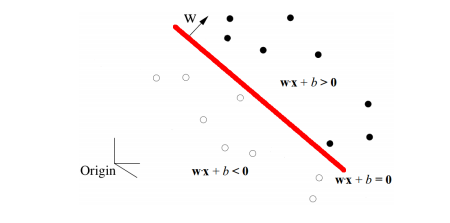
\includegraphics[scale=0.8]{Figs/SVM01.png}
\caption{Hiperplano definido por la ecuación $w\cdot x + b=0$ donde $w$ es la normal y b es el offset, \cite{SebastianGodoy}.}
\label{fig:SVM01}
\end{figure}

Como se observa en la Figura \ref{fig:SVM01} existen dos clases y la forma natural de separar estas clases es hacer una línea la cual tiene una pendiente y un \textit{offset}. Lo que propone el método de SVM es definir esta línea de forma óptima, para encontrar los parámetros $w$ y $b$, tal que la distancia entre los vectores más cercanos a esta línea de cada clase sea la máxima posible. Esto permite que el plano este lo más al medio posible. SVM lo que busca entonces es definir estos dos vectores de forma óptima tal se satisfaga la condición.\\
Se observa además que dos clases diferentes son linealmente separables. La clasificación mediante SVM se obtiene de la siguiente manera a modo de ejemplo.
\begin{equation}
w\cdot x +b > 0 \Rightarrow \hspace{0.5em}  \emph{dato pertenece a clase 0}
\end{equation}
\begin{equation}
w\cdot x +b < 0 \Rightarrow \hspace{0.5em} \emph{dato pertence a clase 1}
\end{equation}

Se observa que la clasificación pasa a ser más sencilla para cada nuevo dato, lo que se tiene que hacer es calcular el producto punto, sumarle el offset y ver el signo del resultado para determinar a qué clase pertenece el dato. Ahora la pregunta más lógica es ¿cuál de las líneas que dividen los hiperplanos es la mejor?
Para dar solución a esta pregunta se propuso que la mejor línea era la que maximizaba el margen, que sería la distancia entre las dos clases.\\
Se llama SVM porque cada uno de los puntos o datos se llaman vectores de soporte, es decir, son los que soportan la definición de la línea. Estos puntos además permiten definir planos $H_{1}$ y $H_{2}$ y la línea optima es la que pasa justo por entremedio de estos dos planos.\\
El problema de optimización es encontrar $w$ y $b$ tal que el margen entre ambos planos $H_{1}$ y $H_{2}$ este maximizado sujeto a la condición de que los vectores deberían estar separados correctamente por el plano tal como se observa a continuación en la Figura \ref{fig:SVM02}.

\begin{figure}[H]
\centering
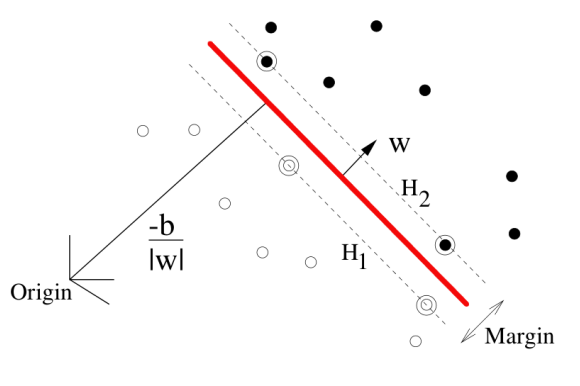
\includegraphics[scale=0.5]{Figs/SVM02.png}
\caption{SVM linealmente separable con sus planos $H_{1}$ y $H_{2}$, \cite{SebastianGodoy}.}
\label{fig:SVM02}
\end{figure}

El margen está determinado por la norma $\frac{1}{\norm{w}}$ y se tiene que tener un set de vectores de entrenamiento definido.\\
SVM además ocupa multiplicadores de Lagrange, esforzándose para encontrar coeficientes tal que:

Buscamos $\alpha_{1},...,\alpha_{n}$ tal que\\

\begin{center}$Q(\alpha)=\sum\limits_{i}\alpha_{i} - \frac{1}{2}\sum\limits_{i}{ \sum\limits_{j}{\alpha_{i}\alpha_{j}y_{i}y_{j}x_{i}x_{j}}}$ este maximizado\\
\end{center}

Sujeto a
\begin{enumerate}
\item[i)] $\sum\limits_{i}{\alpha_{i}y_{i}=0}$
\item[ii)] $\alpha_{i}>=0$ para todo $\alpha_{i}$
\end{enumerate}

Finalmente se define una función y se soluciona la problemática por el producto punto de los vectores de entrenamiento con sus etiquetas.
\begin{equation}
f(x)=\sum \alpha_{i}y_{i}x_{i}\cdot x + b
\label{eq:11}
\end{equation}

Una gran ventaja de este algoritmo es que la implementación se encuentra disponible gracias a \textit{toolboox} en C o en \textit{python} que tienen escritas estas rutinas de optimización.\\
Otro problema ocurre cuando los datos no son separables, es decir, no se puede definir ningún plano. Este problema se resolvió proyectando los datos a otra dimensión donde probablemente, si exista un plano que permite la separación de las clases. Todo se resume en el producto punto de la ecuación \ref{eq:11} que tiene que satisfacer los teoremas antes mencionados. Si no es posible la separación de las clases, pero si la separación es posible en otra dimensión, existe entonces un plano que permite separarlos. Como consecuencia hay un mapeo $\Phi$ que toma el producto punto y lo convierte en el producto punto del mapeo, lo que en realidad define el concepto de kernel que es cualquier función que satisface las condiciones anteriores.\\El kernel implícitamente mapea los datos en un mundo de alta dimensión sin conocer $\Phi$. El kernel lineal que se tenía originalmente para el problema de optimización, se puede definir otro tipo de kernel, como los polinomicos o los Gaussianos, los cuales ocupan combinaciones lineales y el problema de optimización finalmente es el mismo.

%\begin{figure}[H]
%\centering
%\subfigure[]{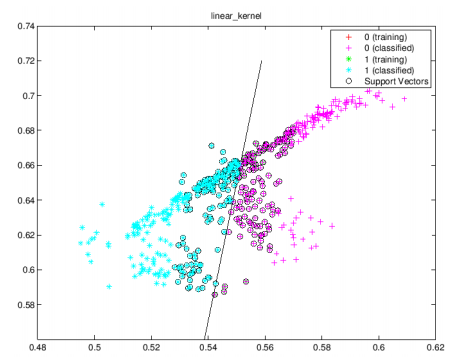
\includegraphics[scale=0.5]{Figs/SVM03.png}}
%\subfigure[]{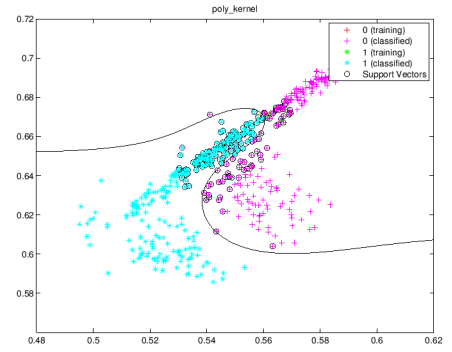
\includegraphics[scale=0.5]{Figs/SVM04.png}}
%\subfigure[]{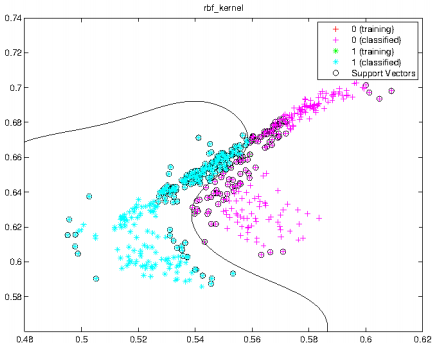
\includegraphics[scale=0.5]{Figs/SVM05.png}}
%\caption{Distintos tipos de kernel para datos de rocas  a) Lineal b) Polinomial c)Guasiano, \cite{SebastianGodoy}.}
%\label{Fig:SVMKernel}
%\end{figure}
Entonces lo que se hace es tomar el problema en cierta dimensión resolverlo linealmente en otra dimensión y después mapearlo de vuelta. Sin lugar a dudas SVM es súper poderoso.

SVM aplicado a rostros computacionalmente es costoso en la etapa de entrenamiento, pero una vez que se realiza esta etapa, es el cálculo de multiplicar productos puntos y sumas lo hace sencillo. Otro problema que se ve es que si se ingresa una nueva cara a la base de datos es necesario entrenar de nuevo.\\
 Finalmente como conclusión de este método podemos decir que en términos de aplicabilidad, una vez que ya se está entrenado, es comparable con el algoritmo de Eigenface.

\newpage
\subsubsection{Evaluación de algoritmos de reconocimiento facial propuestos por Inostroza}

La idea es explicar de manera más detallada cada algoritmo estudiado por Inostroza \cite{ElectronicoUdeC}. Primero aclarar que el conjunto de imágenes utilizado para realizar las pruebas de reconocimiento corresponde a una base de datos que contiene cuatrocientos rostros de cuarenta individuos distintos, y que pertenece a la base de datos {\textit{Olivetti Research Laboratory}}.\\


%Los resultados de sistemas de reconocimiento de rostros, se ve dificultado debido a la amplia variedad de conjunto de imágenes, cantidad de éstas y normalización, etc.
\paragraph{Comparación con plantilla (Template Matching)}

Este método busca a partir de un conjunto de imágenes, tener definidas distintas  clases, en otras palabras, una clase es un \textit{set} de imágenes de un individuo. A partir de cada clase entonces se creará a lo menos una plantilla o máscara para que una vez que llegue la nueva imagen a clasificar, se mida la distancia entre la plantilla de la nueva imagen, con cada plantilla de las diferentes clases antes obtenidas. La forma de crear una plantilla es usar el promedio entre todas las imágenes o usar la características principales de la clase y se obtiene algo como la Figura \ref{fig:PantillaAS}.
\begin{figure}[H]
\centering
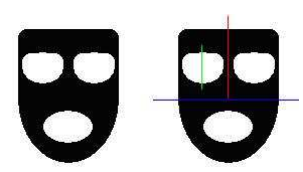
\includegraphics[scale=0.5]{Figs/Plantilla.png}
\caption{Plantillas usadas para la detección de rostros, \cite{AmirFa}.}
\label{fig:PantillaAS}
\end{figure}

La comparación con una plantilla entonces se refiere a medir directamente la distancia entre un patrón de entrada y aquellos almacenados en la base de datos, para permitir la correspondencia de cada patrón presentado. Los patrones son considerados como vectores y la correspondencia de cada patrón de entrada, con otra base de datos, se realiza con base en la menor distancia encontrada entre estos \cite{bunschoten}.\\
El método de comparación con una plantilla es un sistema de clasificación de patrones que consiste en determinar cuál de las clases almacenadas en la base de datos se encuentra más cercana, utilizando una medida dada, al patrón de entrada presentado. Dado un vector de entrada $x$ y un conjunto de vectores de referencia (plantillas) $m_{i}$, se busca el vector $m_{c}$ tal que

\begin{equation}
    \norm{ x - m_{c} } = 
            min_{i}{\norm{x-m_{i}}}  \hspace{1cm} x,m_{i} \in \Re
\end{equation}

La norma utilizada para la medición entre los patrones es arbitraria, pudiendo usarse la norma euclidiana. A priori se puede ver que el éxito radica en que los patrones presentados en la entrada, tengan la mayor similitud posible con su respectiva base de datos, tanto en lo que se refiere a tamaño, ubicación, orientación, intensidad, dirección de la iluminación. El método tiene fallos, por ejemplo, si el tamaño de la plantilla es diferente al de la imagen nueva el método no funciona (ver Figura \ref{fig:Mascaras}) o si cambia el fondo de la imagen a detectar. Tampoco funciona si se cambia la rotación del rostro o hay cambios en la iluminación en la imagen. Debido a todo lo mencionado no es factible utilizar este método e implementarlo en la Raspberry Pi debido a lo limitado del algoritmo.

\begin{figure}[H]
\centering
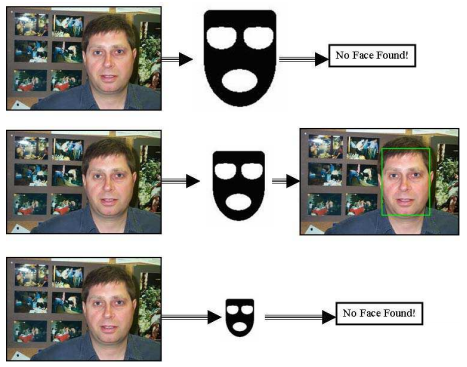
\includegraphics[scale=0.5]{Figs/DifferentSizeModes.png}
\caption{Errores al implementar distintos tamaños de plantillas o máscaras, \cite{AmirFa}.}
\label{fig:Mascaras}
\end{figure}


\paragraph{Mapas Auto-Organizativos}

Es un tipo de red neuronal que se caracteriza por preservar las similitudes en los patrones de entrada como similitudes en la localización topológica de la salida.\\
Se asimila mucho a la idea de Eigenface ya que se tienen estas métricas buscando la similitud entre los rostros a través de las características principales. 
En el mapa auto-organizativo, cada una de las células se sintoniza específicamente a cierto patrón o clase de patrón de entrada. Este es presentado a todas las células, y la magnitud de la respuesta que una de ellas entregue dependerá de cuanta similitud exista entre el vector de referencia de la célula en particular con el patrón de entrada. La célula más sintonizada con una entrada determinada(denominada célula ``ganadora''), emitirá la mayor señal de salida, mientras que las células vecinas presentarán señales de salida menores, disminuyendo su magnitud a medida que se encuentran más alejadas de la célula ``ganadora'' \cite{ElectronicoUdeC} . 
Este tipo de algoritmo es especialmente útil en la clasificación de datos que presentan a un gran número de clases.\\
La utilización de mapas auto-organizativos en el reconocimiento de rostros pretende que el algoritmo aprenda la distribución de probabilidad de un conjunto de imágenes de entrenamiento y ordene los vectores de referencia de los nodos, de tal forma que permita que imágenes no utilizadas en el entrenamiento, pero que pertenecen a individuos conocidos, puedan ser identificadas de la mejor forma posible. La principal desventaja haciéndolo poco aplicable al problema del proyecto es que el entrenamiento puede durar hasta un día y medio usando la base de datos {\textit{Olivetti Research Laboratory}.}

\paragraph{Bases de características no ortogonales}

Este algoritmo se basa en mapas auto-organizativos, que tiene como finalidad crear una base de características no ortogonales para la representación de un conjunto de datos vectoriales. Se pretende crear una base no orgonal de características, que represente en forma adecuada un cierto conjunto de vectores. Al igual que el algoritmo anterior su desventaja es la etapa de entrenamiento.


\paragraph{Resultados obtenidos de los tres algoritmos}

Cabe destacar que las imágenes trabajadas por Inostroza  \cite{ElectronicoUdeC}, son de fondo controlado, en las que el rostro se encuentra medianamente normalizado en cuanto a orientación y posición.\\
La comparación de rostros con plantilla, ha sido el que ha arrojado los mejores porcentajes de reconocimiento, llegando a reconocer en los mejores casos, 199 imágenes de las 200 que le han sido presentadas para la clasificación. Las imágenes pertenecen a 40 individuos diferentes (utilizandose como referencia 5 imágenes de cada uno).\\
Incluso al utilizar imágenes de baja resolución (23x28 píxeles), y el conjunto seleccionado manualmente, se obtiene un buen porcentaje de reconocimiento con un promedio de $95.25\%$. La velocidad de reconocimiento relativamente alta (0.515 segundos por imagen en el caso más lento cuando se utiliza una resolución de de 23x28 píxeles).\\
Para el segundo algoritmo, la utilización de mapas auto-organizativos, presenta un desempeño menor al algoritmo de comparación de plantillas en casi todos los sentidos. La necesidad de este método de que los vectores de referencia sean creados mediante entrenamiento, es su principal desventaja, ya que tarde demaciado tiempo volviendo el método impráctico.\\
Para el tercer algoritmo bajo evaluación por Inostroza \cite{ElectronicoUdeC} arrojan resultados que están por debajo de los obtenidos por los dos algoritmos anteriores. La desventaja es que el tiempo de entranamiento es aproximadamente 7.15 veces superior al mapa auto-organizativo. En resumen se obtuvo los resultados que se muestran en la siguiente tabla \ref{TablaInostroza}

\begin{table}[H]
\begin{tabular}{|c|c|c|c|}
\hline 
\multicolumn{4}{|c|}{Porcentaje de reconocimiento} \\ 
\hline 
Método&Comparación con plantilla&Mapa auto-organizativo&Base características no ortogonales\\ 
\hline 
$\%$Máximo& 99$\%$ & 97$\%$& 87.5$\%$ \\ 
\hline 
\multicolumn{4}{|c|}{Tiempo de reconocimiento(200 imágenes)} \\ 
\hline 
Método&Comparación con plantilla&Mapa auto-organizativo&Base características no ortogonales\\ 
\hline 
Segundos& 1 a 713 [seg] & 2 a 4 [seg]& 4 [seg] \\ 
\hline 
\end{tabular}
\caption{Desempeños de algoritmos}
\label{TablaInostroza} 
\end{table}
% ***********************************************************************************
% ***********************************************************************************
\newpage
\subsection{Simulaciones preliminares.}
\subsubsection{Simulación distancia Euclidiana en Matlab}
Para la base de datos elegida se implemento la clasificación de mínima distancia Euclidiana (en adelante lo referimos como clasificador Euclidiano).
\begin{figure}[H]
\centering
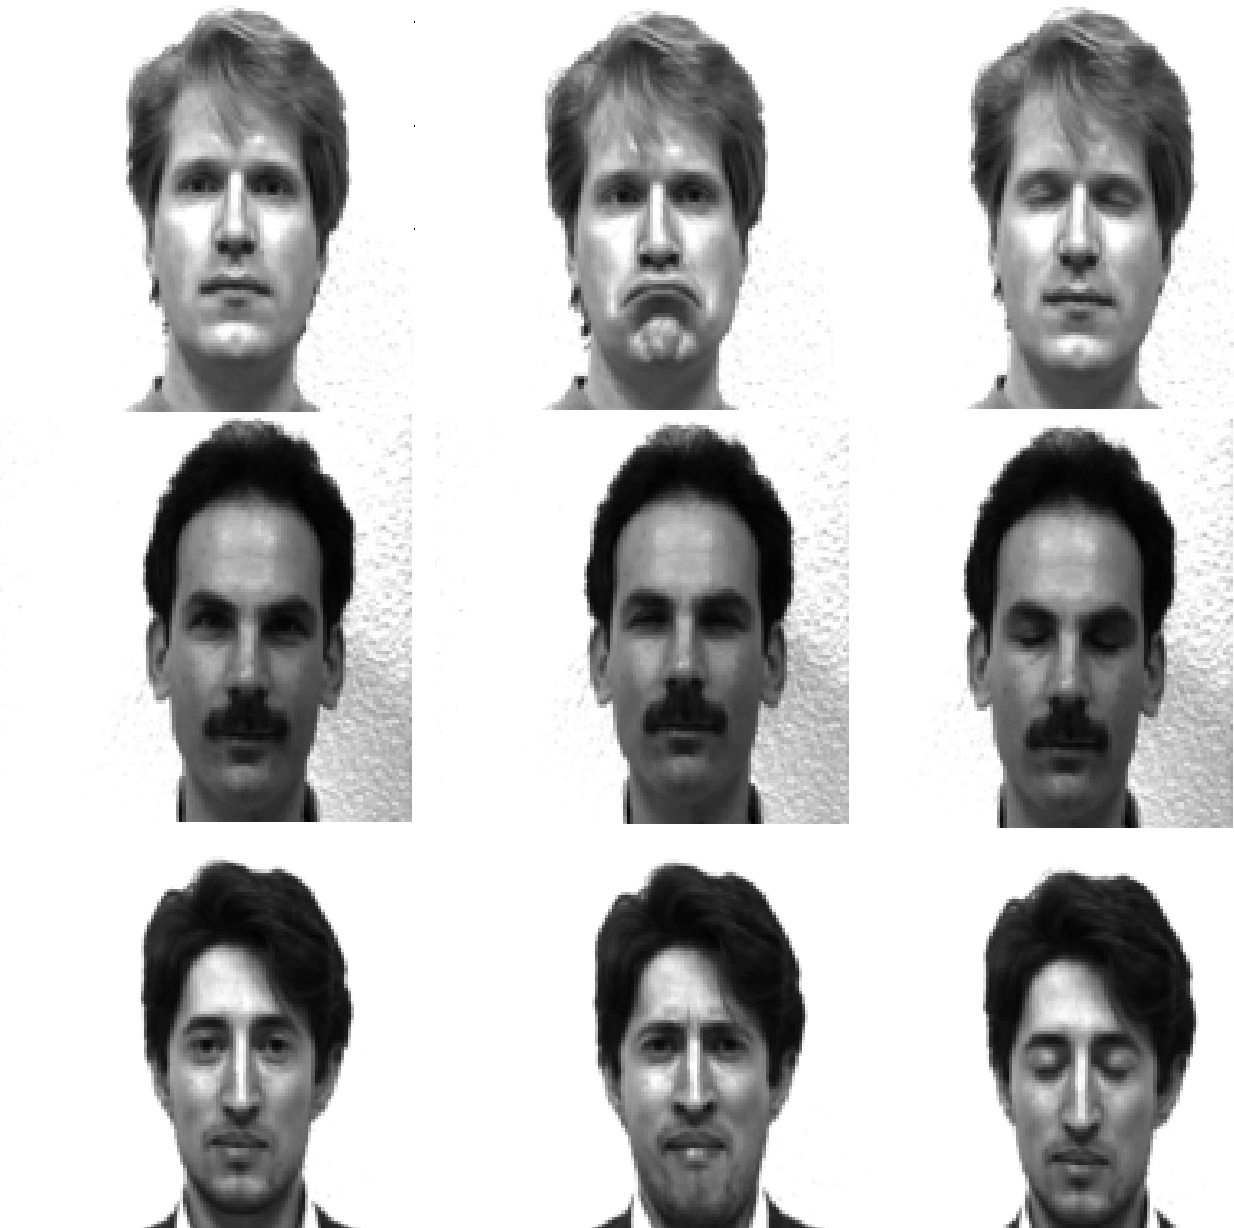
\includegraphics[scale=0.3,keepaspectratio=true]{Figs/BasedeDatosEu.png}
\caption{Base de datos YaleFace con 3 sujeto en 3 distintas situaciones.}
\label{Fig:BasedeDatos}
\end{figure}

\begin{figure}[h]
\centering
\subfigure[]{ 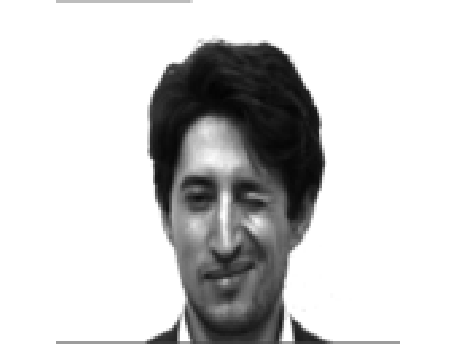
\includegraphics[scale=0.44,keepaspectratio=true]{Figs/ImagendePruebaEu.png}}
\subfigure[]{ 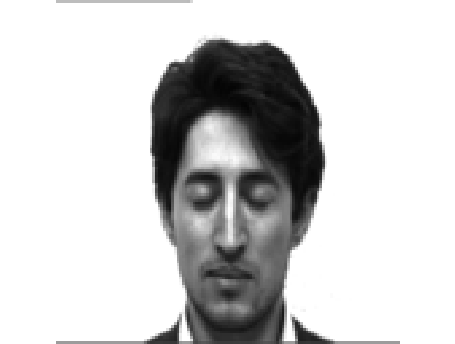
\includegraphics[scale=0.44,keepaspectratio=true]{Figs/ClasificadoEu.png}}
\caption{a) Imagen de Prueba b)Sujeto detectado con mínima distancia Euclidiana.}
\label{fig:2}
\end{figure} 
% ***********************************************************************************
% ***********************************************************************************
\vspace{1cm}
Entonces,  observe la Figura~\ref{Fig:BasedeDatos}. En esta figura, se muestra
la pequeña base de datos correspondientes a yaleface de 3 sujetos. De los resultado se esperaba un peor comportamiento, ya que la distancia Euclidiana solo  dice a cual sujeto se parece más la imagen de prueba. Es decir si tenemos dos sujetos que se parecen la distancia Euclidiana no necesariamente va a elegir al sujeto correcto.
\vspace{1cm}
% ***********************************************************************************
% ***********************************************************************************

\subsubsection{Simulación Eigenface en Matlab}
Se trabajo con la misma base de datos.
\begin{figure}[H]
 \centering
 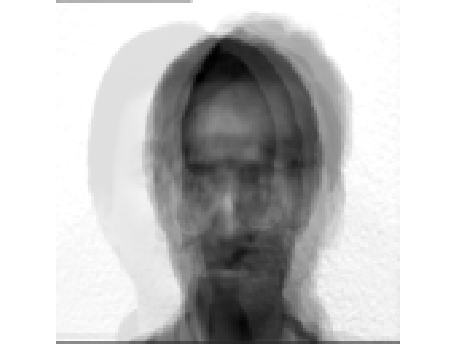
\includegraphics[scale=0.3,keepaspectratio=true]{Figs/PromedioEi.png}
\caption{Cálculo de rostro promedio.}
 \label{Fig:Prom}
\end{figure}


\begin{figure}[H]
 \centering
 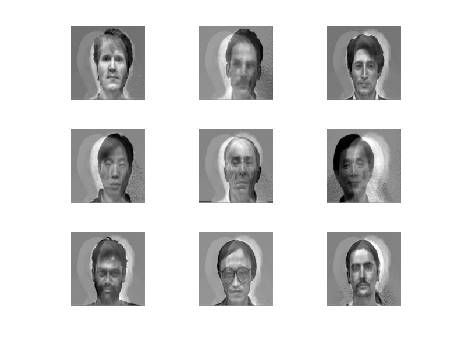
\includegraphics[scale=0.95,keepaspectratio=true]{Figs/RestaPromEi.png}
\caption{Resta del rostro promedio a cada una de las imagenes.}
 \label{Fig:ResProm}
\end{figure}

\begin{figure}[H]
 \centering
 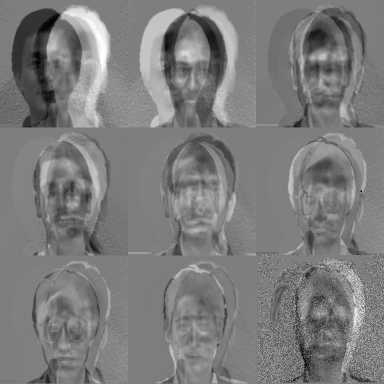
\includegraphics[scale=0.9,keepaspectratio=true]{Figs/Eigenfaces.png}
\caption{Eigenfaces.}
 \label{Fig:Eigenfaces}
\end{figure}

\begin{figure}[h]
\centering
\subfigure[]{ 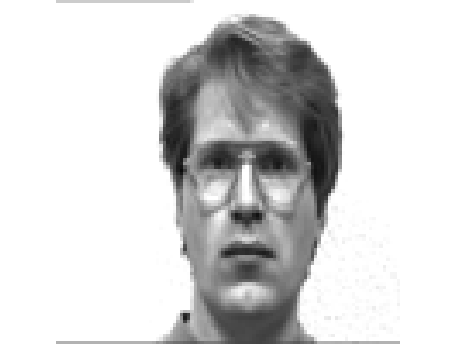
\includegraphics[scale=0.48,keepaspectratio=true]{Figs/ImagenAdetectarEi.png}}
\subfigure[]{ 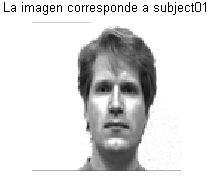
\includegraphics[scale=0.78,keepaspectratio=true]{Figs/clasificadaEi.png}}
\caption{a) Imagen de Prueba b)Sujeto detectado con algoritmo \emph{Eigenface}.}
\label{fig:2}
\end{figure} 

Como se observa  en la simulación de \emph{Eigenface} se aplicaron los algoritmos antes descritos y sus respectivos cálculos matemáticos. 
\newpage
\subsection{Raspberry Pi}
\subsubsection{Hardware Raspberry Pi}
\label{HardLim}
Debido a que se ha comentado del hardware limitado de la tarjeta comercial Raspberry Pi se expondrá cual son sus componentes en hardware.\\
El diseño incluye un \textit{system-on-a-chip Broadcom BCM2835}, que permite hacer overclocking hasta velocidad Turbo; 1000 MHz ARM, 500 MHz core, 600 MHz SDRAM, 6 overvolt. de forma segura. Contiene un procesador central de 700MHz \textit{ARM1176JZF-S core} con una \textit{GPU Broadcom VideoCore IV, OpenGL ES 2.0, OpenVG 1080p30 H.264 / MPEG-4 AVC} de alto perfil decodificador y una memoria \textit{SDRAM} de 512 Megabytes. La primera Raspberry al ser lanzada tenia solamente 256 Megabytes de SDRAM. El modelo que se utilizó para este proyecto incluye cuatro puertos USB con un puerto de red Ethernet tal como se observa a continuación en la Figura \ref{Fig:Rpi}.

\begin{figure}[H]
\centering
\subfigure[]{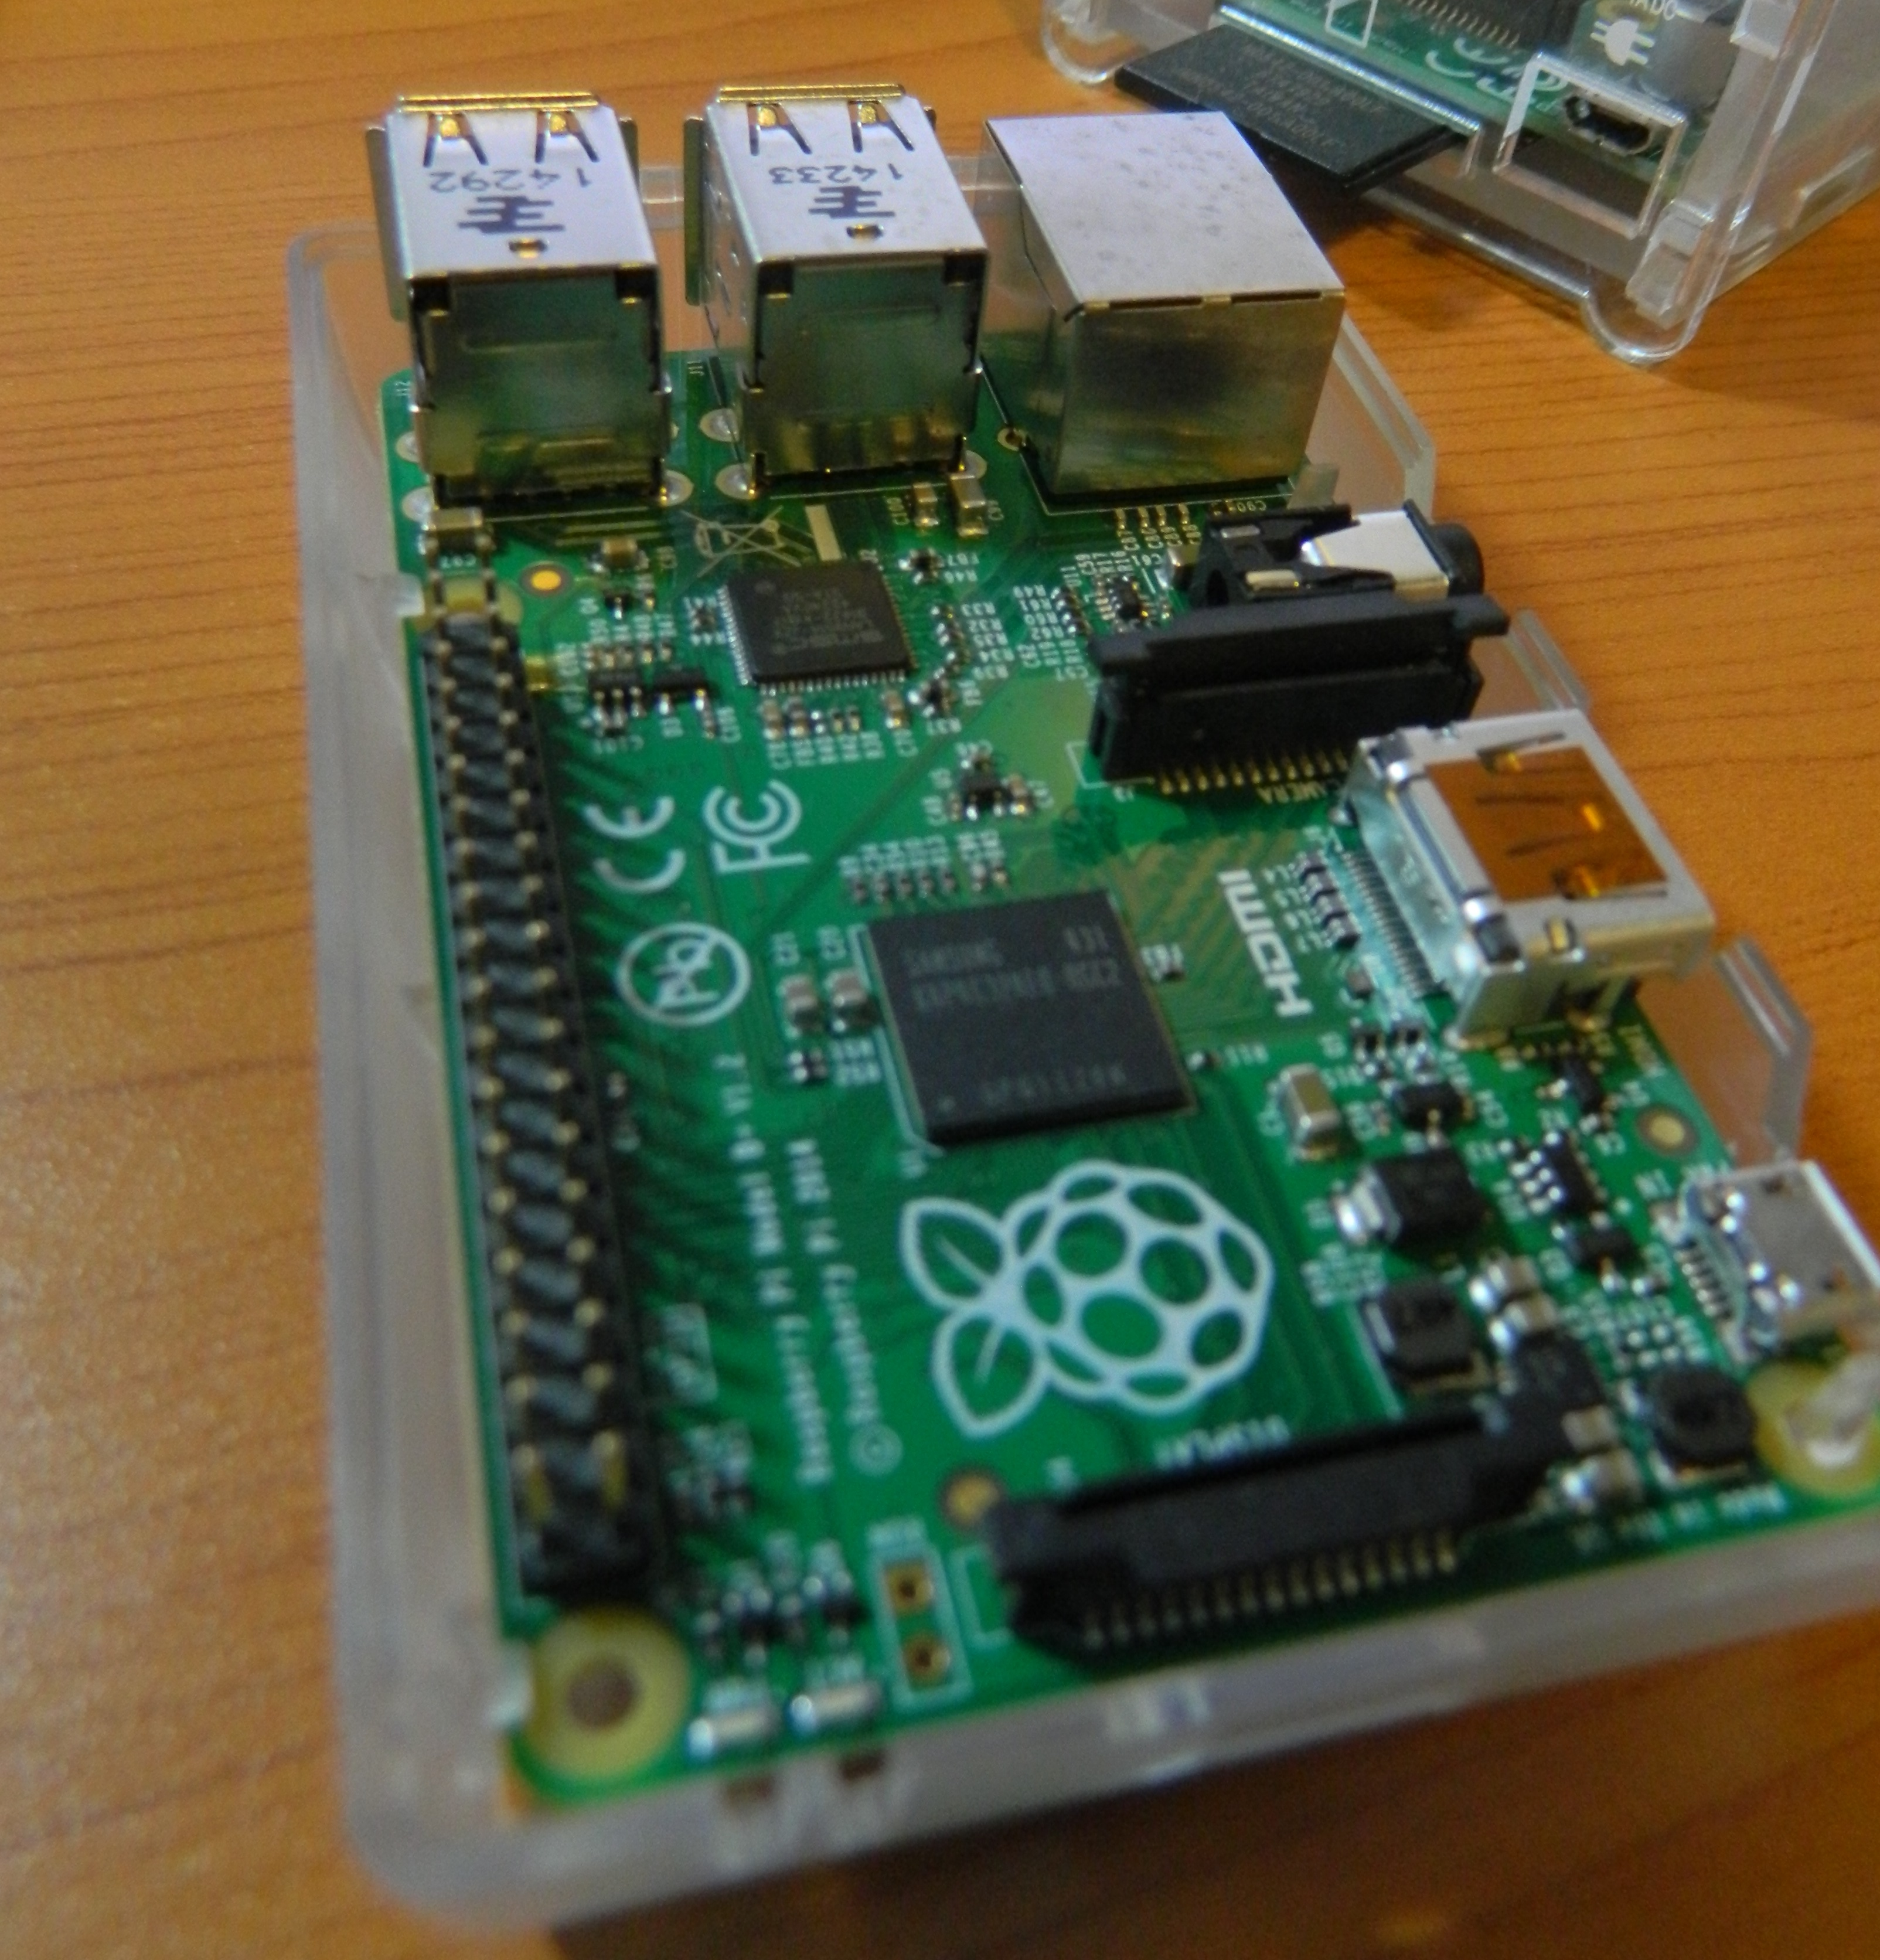
\includegraphics[scale=0.15]{Figs/Rpi1.jpg}}
\subfigure[]{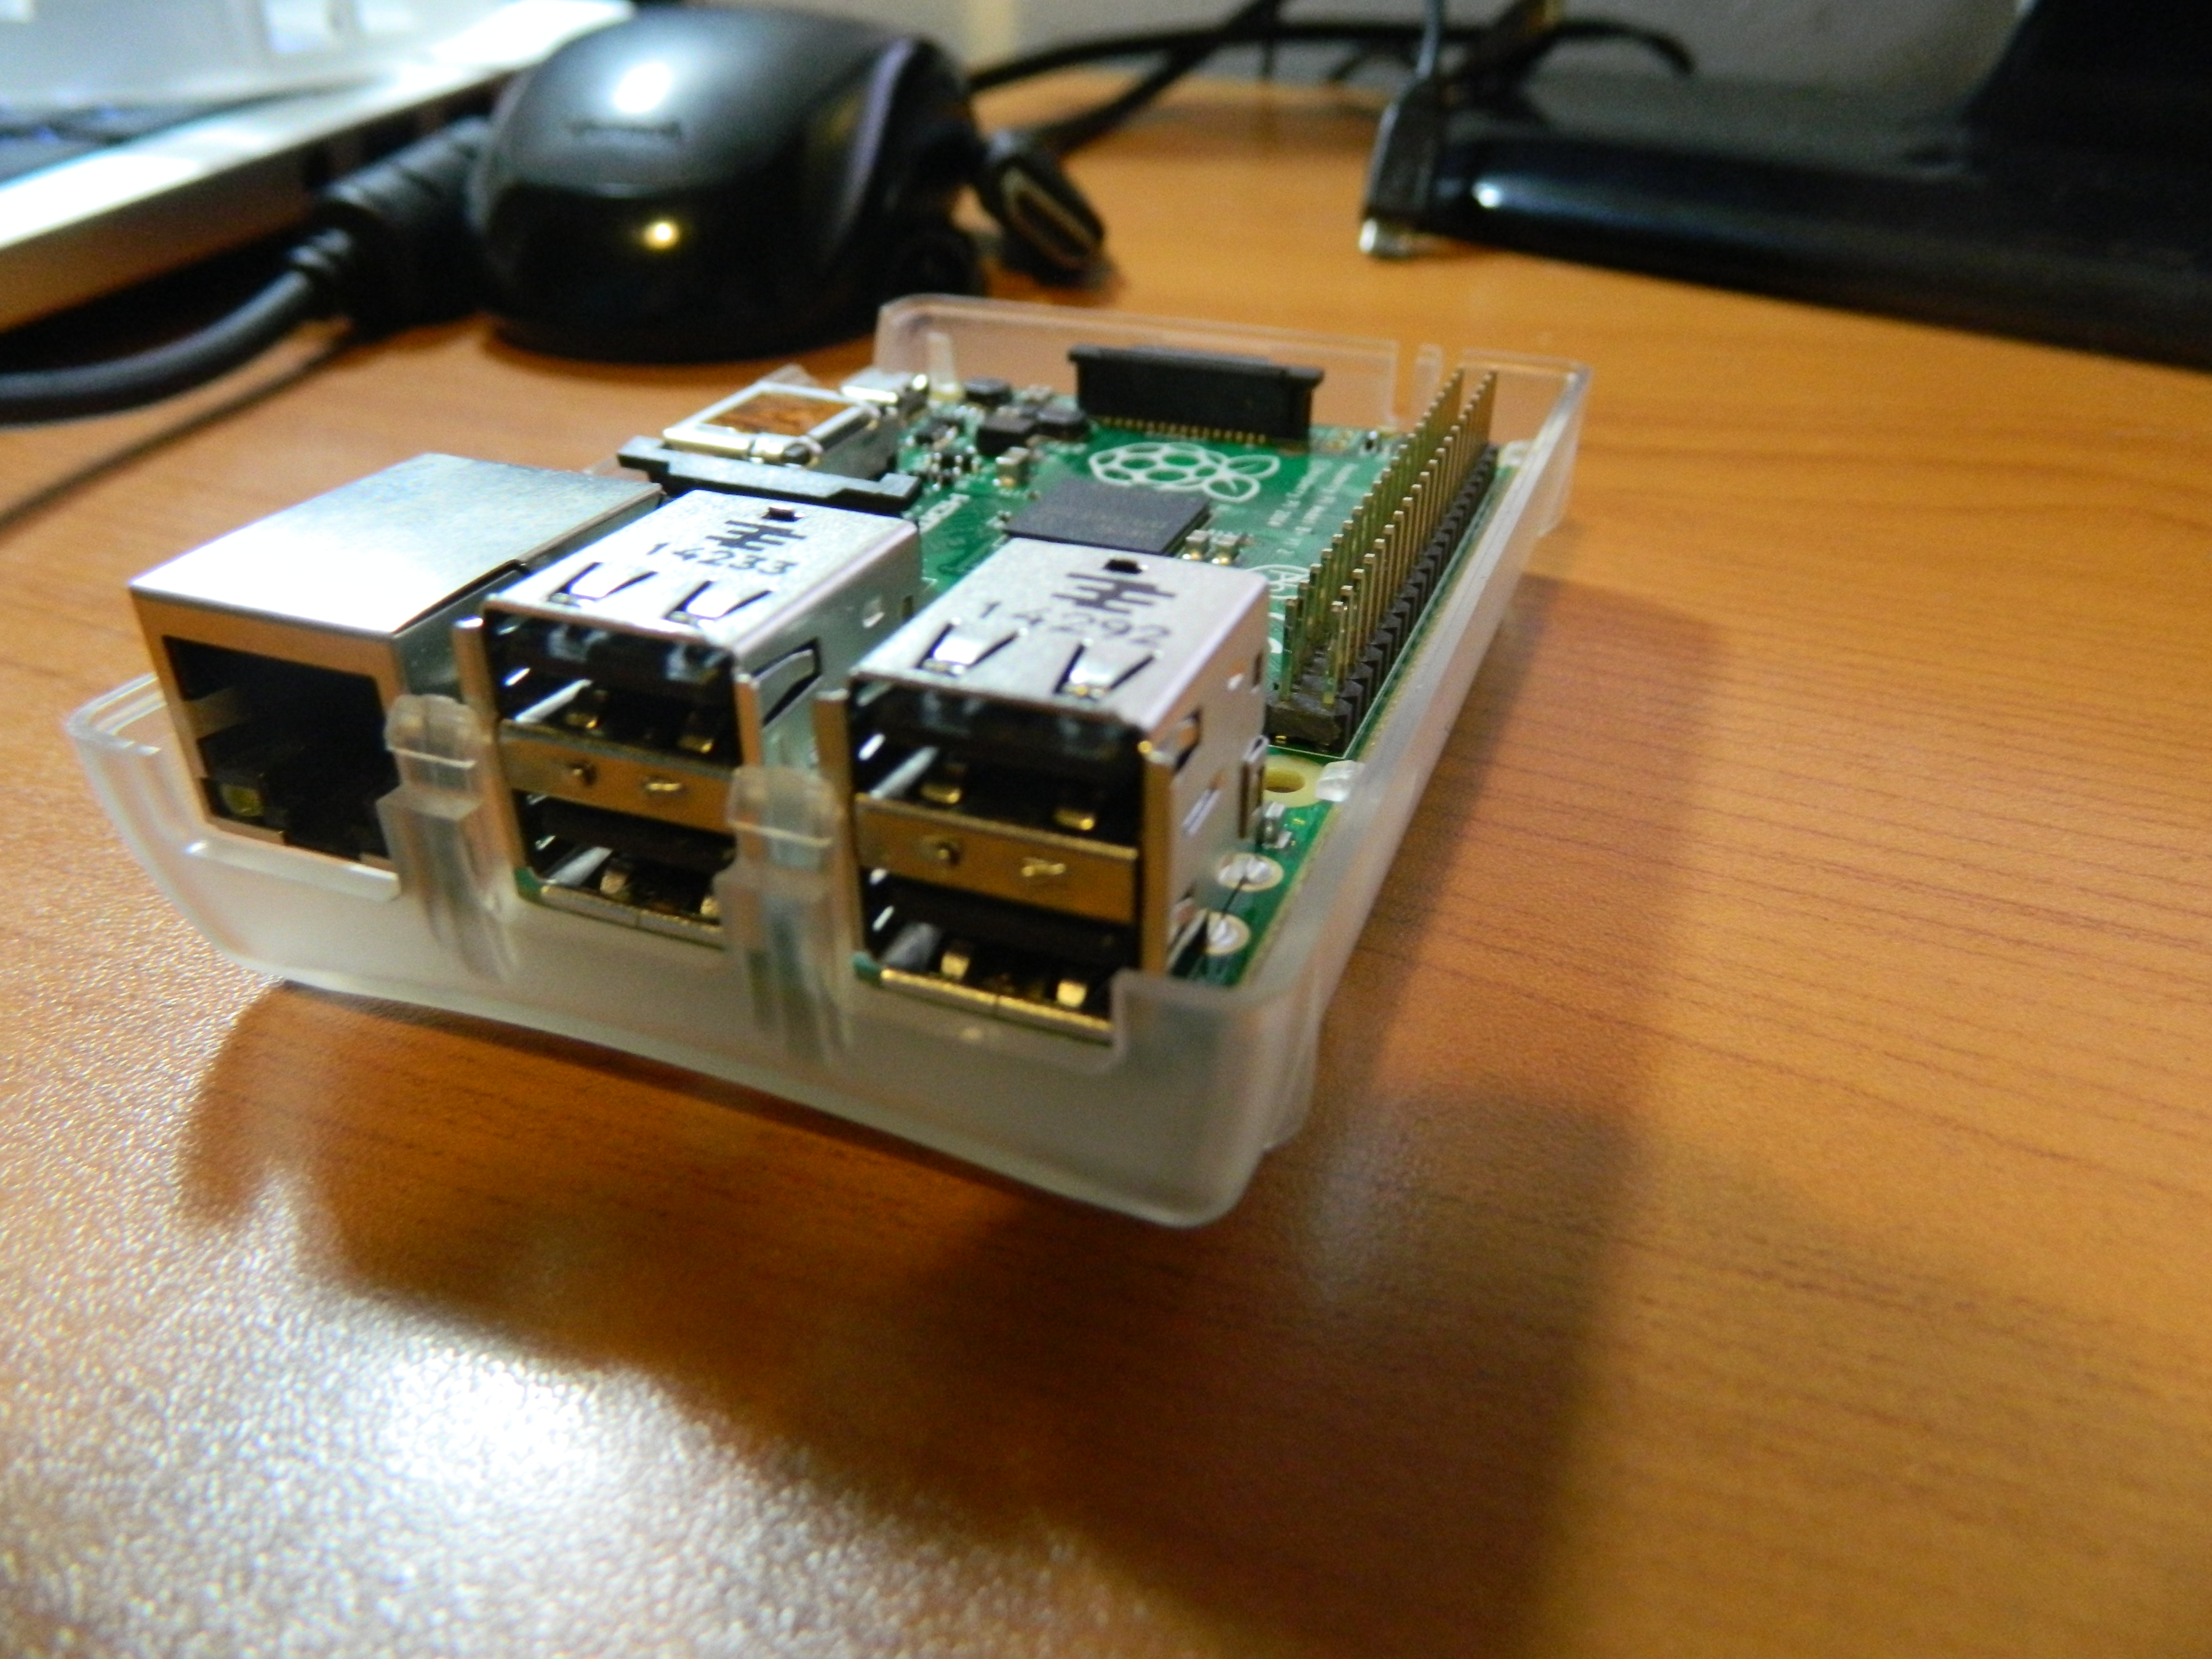
\includegraphics[scale=0.037]{Figs/Rpi2.jpg}}
\subfigure[]{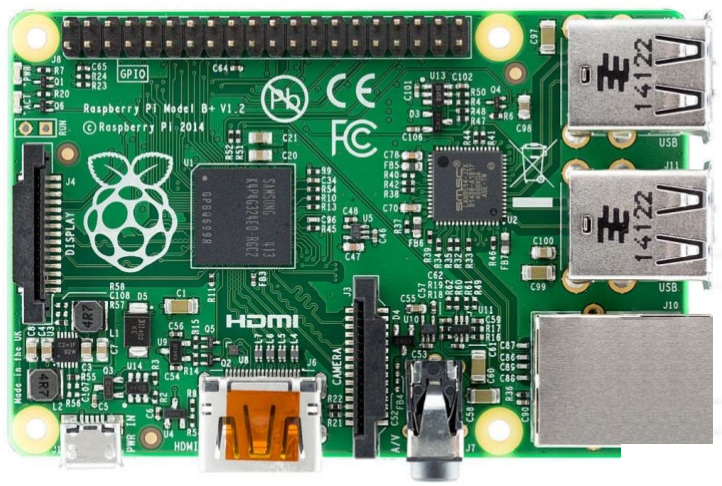
\includegraphics[scale=0.3]{Figs/Rpi3.png}}
\caption{Hardware de Raspberry Pi utilizada para realizar este proyecto}
\label{Fig:Rpi}
\end{figure}


El diseño no incluye un disco duro o una unidad de estado sólido, ya que usa una tarjeta micro SD para el almacenamiento permanente;tampoco incluye fuente de alimentación\cite{TrabajoRaspiUdeC}.\\
Respecto a los periféricos, la tarjeta se puede visualizar en una TV o monitor gracias a la conexión HDMI @ 1920x1200 píxeles. Se puede conectar una cámara, lo cual puede ser una WebCam o la Raspberry Pi Cam. También posee una conexión ethernet 10/100 Mbps para proveer de una conexión a internet o se puede obtener un Wi-Pi que es una adaptar USB de WiFi. Por último los perifericos más utilizados con un teclado y mouse USB que permiten el manejo y darle instrucciones a las Raspberry Pi. En la Figura \ref{Fig:ComponentesRpi} se puede observar los periféricos más relevantes.
\begin{figure}[H]
\centering
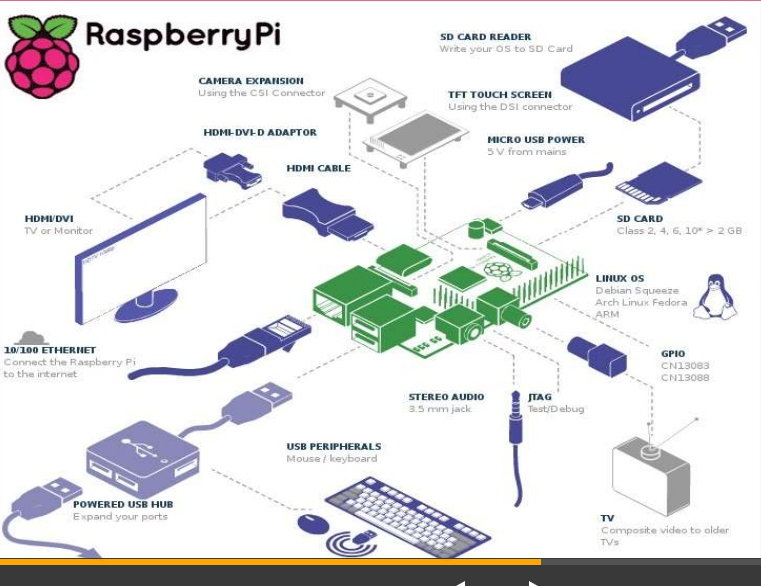
\includegraphics[scale=0.3]{Figs/Perifericos.png}
\caption{Todos los periféricos que se pueden conectar a la Raspberry Pi Modelo B, de dos puertos USB,\cite{HardwarePiPeri}.}
\label{Fig:ComponentesRpi}
\end{figure}


El tamaño de esta placa es de $85,60x56,5mm$ con un peso de $45$ g y un consumo de energía de $5v, 600mA$. 





\subsubsection{Pi Cam}

La instalación de la Pi cámara esta muy bien explicado por el CEO en el sitio oficial de Raspberry Pi \url{http://www.raspberrypi.org/archives/3890}.\\
Gracias a la carcasa de la Raspberry Pi, la cámara queda bien montada en la tarjeta y la cinta flex queda protegida, disminuyendo los riesgos por estática. El último paso para montar la cámara es atornillada a la carcasa dejando bien asegurada. La Pi cam y como quedó montada se pude observar en la Figura \ref{fig:Campi}.\\
Para activar la cámara basta con entrar a la configuración de la Raspberry Pi y navegar hasta cámara para seleccionar \textit{``enable"}. 

\begin{figure}[H]
\centering
\subfigure[]{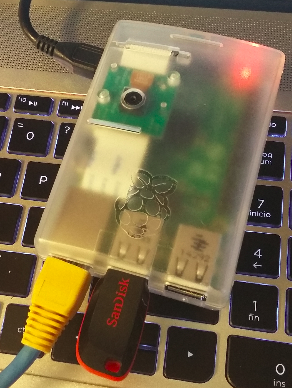
\includegraphics[scale=0.3,keepaspectratio=true]{Figs/Picam1.png}}
\subfigure[]{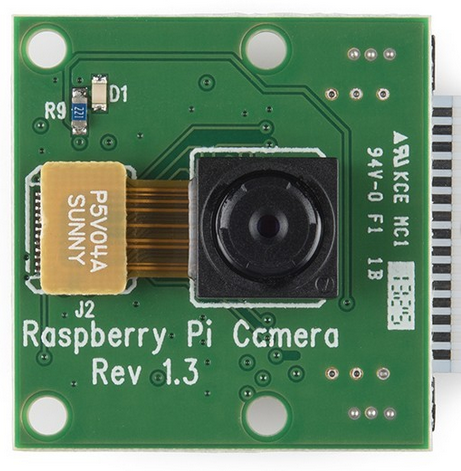
\includegraphics[scale=0.3,keepaspectratio=true]{Figs/Picam2.png}}
\subfigure[]{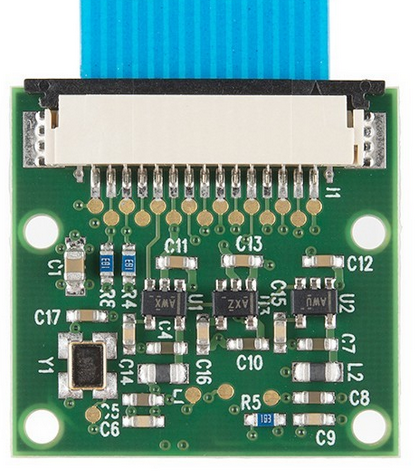
\includegraphics[scale=0.3,keepaspectratio=true]{Figs/Picam3.png}}
\subfigure[]{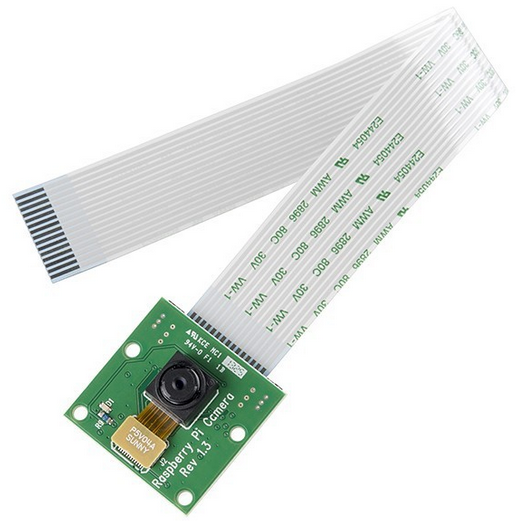
\includegraphics[scale=0.3,keepaspectratio=true]{Figs/Picam4.png}}
\caption{a)Raspberry Pi con carcasa y Pi Cam montada b)c)d)Imágenes de cámara Raspberry Pi que se utiliza en el proyecto, \cite{ImagenesPiCam}}
\label{fig:Campi}
\end{figure}






\subsubsection{Instalación de OpenCV en Raspberry Pi}

El proceso para instalar OpenCV tomó alrededor de 10 horas. Esto se debe a la creación de un código OpenCV configuración y construcción \cite{RoboPapa}.\\
Como con cualquier instalación en el Raspberry Pi, se comienza con la actualización de está con el siguiente comando:\\

\begin{lstlisting}[language=bash, frame=single]
sudo apt-get update
\end{lstlisting}
\begin{figure}[H]
\centering
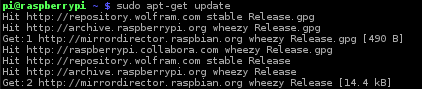
\includegraphics[scale=0.6,keepaspectratio=true]{Figs/Raspy1.png}
\caption{Update solo chequea repositorios. }
\label{fig:Raspy1}
\end{figure}

\begin{lstlisting}[language=bash, frame=single]
sudo apt-get upgrade
\end{lstlisting}

\begin{figure}[H]
\centering
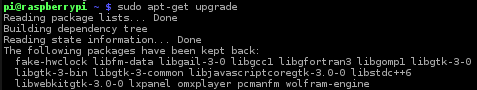
\includegraphics[scale=0.6,keepaspectratio=true]{Figs/Raspy2.png}
\caption{Upgrade ejecuta la actualizacion efectiva del sistema.}
\label{fig:Raspy2}
\end{figure}

Luego se ejecutan los dos comandos siguientes:
\begin{lstlisting}[language=bash, frame=single]
sudo apt-get -y install build-essential cmake cmake-curses-gui\
pkg-config libpng12-0 libpng12-dev libpng++-dev libpng3\
libpnglite-dev zlib1g-dbg zlib1g zlib1g-dev pngtools \
libtiff4-dev libtiff4 libtiffxx0c2 libtiff-tools\
libeigen3-dev
\end{lstlisting}

\begin{lstlisting}[language=bash, frame=single]
sudo apt-get -y install libjpeg8 libjpeg8-dev libjpeg8-dbg\
libjpeg-progs ffmpeg libavcodec-dev libavcodec53 libavformat53\
libavformat-dev libgstreamer0.10-0-dbg libgstreamer0.10-0\
libgstreamer0.10-dev libxine1-ffmpeg libxine-dev libxine1-bin\
libunicap2 libunicap2-dev swig libv4l-0 libv4l-dev python-numpy\
libpython2.6 python-dev python2.6-dev libgtk2.0-dev
\end{lstlisting}
Después de que las bibliotecas hayan terminado de instalar. Luego se descarga la versión de OpenCV 2.4.9 utilizando el comando wget para descargar el archivo zip 
\begin{lstlisting}[language=bash, frame=single]
wget -O openCV-2.4.9.zip\
http://sourceforge.net/projects/opencvlibrary/files/opencv\
-unix/2.4.9/opencv-2.4.9.zip/download
\end{lstlisting}
Después de finalizada la descarga se tendrá openCV-2.4.9.zip, el paso siguiente es utilizar el comando unzip para descomprimir el archivo zip
\begin{lstlisting}[language=bash, frame=single]
unzip openCV-2.4.9.zip 
\end{lstlisting}
Esto creará una carpeta OpenCV-2.4.9. Se creá la carpeta realease que es donde vamos a compilar OpenCV.
\begin{lstlisting}[language=bash, frame=single]
cd openCV-2.4.9
mkdir release
cd release
\end{lstlisting}

Luego es el momento de configurar OpenCV. Se trata de una larga lista, la cual se puede configurar o usar como viene por defecto. Para entrar al menú de configuración escribimos lo siguiente.
\begin{lstlisting}[language=bash] 
sudo ccmake ../ 
\end{lstlisting}

\begin{figure}[H]
\centering
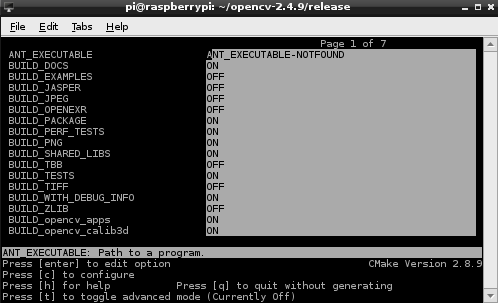
\includegraphics[scale=0.5,keepaspectratio=true]{Figs/Raspy04.png}
\caption{Configuración OpenCV.}
\label{fig:Raspy3}
\end{figure}

Una vez terminada la configuración y guardada, se comenzó a ejecutar el siguiente comando: (estos comandos tomaron alrededor de 10 horas).
\begin{lstlisting}[language=bash, frame=single]
make
sudo make install
\end{lstlisting}

En este punto se ha terminado exitosamente de instalar OpenCV. 

\subsubsection{Problemas con la instalación OpenCV}

Una problemática en la instalación de OpenCV es la capacidad del la tarjeta micro SD. Esta es de 8GB y al terminar de instalar OpenCV queda ocupado alrededor de un 85\% de la capacidad total de memoria de la Raspberry Pi. \\
En una primera instancia, el Makefile generado con los archivos de proyecto, los archivos objeto y binarios de salida ocuparon el 100\% de capacidad de la Raspberry Pi. Se intentó con comandos liberadores de espacio {\tt sudo apt-get clean } y {\tt sudo apt-get autoremove }. La consecuencia de utilizar estos comandos es que eliminan todos los paquetes del cache y borra los paquetes huérfanos produciendo un error ya que la Raspberry no funcionó correctamente y el espacio liberado no fue significativo. La solución al problema fue reinstalar todo desde el sistema operativo Raspbian desde cero hasta OpenCV y montar un pendrive de 16GB a la Raspberry con la finalidad de evitar problemas de espacio.

\subsubsection{Implementación de Eigenface con OpenCV en la Raspberry Pi}

Se siguió con dificultades el tutorial disponible en \url{https://thinkrpi.wordpress.com/opencv-and-pi-camera-board/}.\\
 El proyecto consiste en desarrollar un sistema de visión embebido, capaz de detectar rostros de sujetos presentes en la base de datos. Este tutorial aún no se termina y lo que hace básicamente es modificar el código fuente de una implemetación anterior realizada por el mismo autor, pero utilizando una WebCam.\\
 Es necesario descargar la API de reconocimiento facial que está implementada en OpenCV de \url{https://github.com/raspberrypi/userland}. Se extrae y se compila con los siguientes comandos:
 
\begin{lstlisting}[language=bash, frame=single]
sudo cmake .
sudo make 
\end{lstlisting}
 
 Los resultados luego de terminar el paso 2 del tutorial son:
 
\begin{figure}[H]
\centering
\subfigure[]{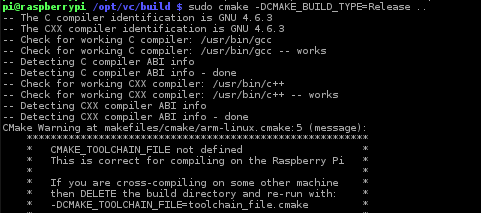
\includegraphics[scale=0.6]{Figs/Paso01.png}}
\subfigure[]{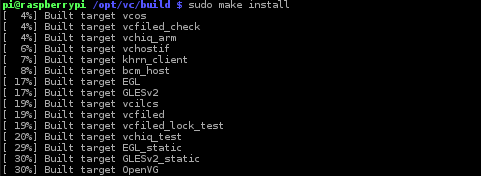
\includegraphics[scale=0.72]{Figs/Paso02.png}}
\subfigure[]{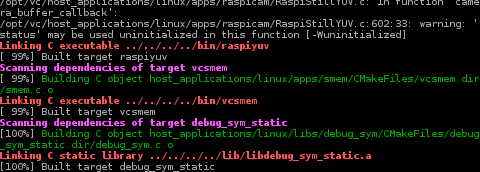
\includegraphics[scale=0.7]{Figs/Paso03.png}}
\caption{Creación y construcción del directorio con el que se trabaja.}
\label{Fig:Paso2Turto}
\end{figure}
 
 En el paso 6 la capturación del vídeo se obtuvo el siguiente resultado:
 
\begin{figure}[H]
\centering
\subfigure[]{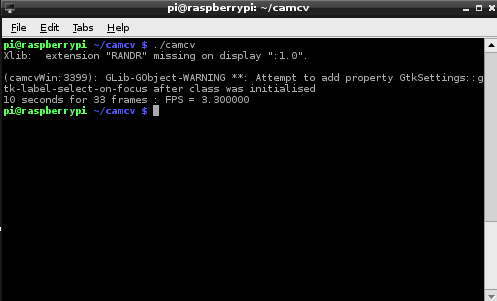
\includegraphics[scale=0.6]{Figs/Step6Resultados2Nuevo.png}}
\subfigure[]{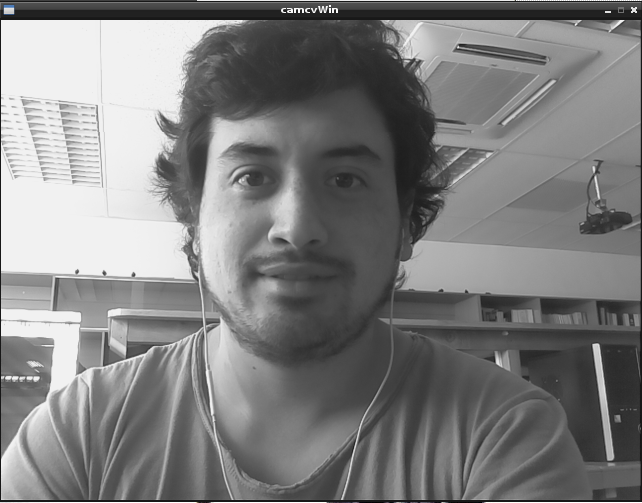
\includegraphics[scale=0.36]{Figs/Step6Resultados.png}}
\caption{a) Ejecución del programa luego de construir y compilar b)Devolución de un video a 30 FPS capturado en Laboratorio de Redes de Datos.}
\label{Fig:Video}
\end{figure}
 
 Lamentablemente con cuatro días de intento para dar la soluciones de los errores de compilación del paso 7 no se pudo terminar este tutorial completamente. Lo que se busca es el siguiente resultado.
 
\begin{figure}[H]
\centering
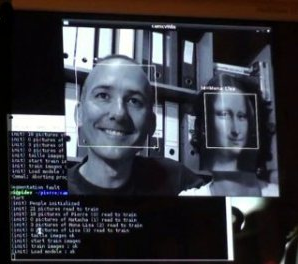
\includegraphics[scale=0.8]{Figs/Paso7.png}
\caption{Resultado esperado al término del tutorial}
\label{Fig:Thinki}
\end{figure} 
 
\subsubsection{Segmentación de Rostros}
 
 El rostro humano es muy dinámico y puede tomar distintas apariencias. A un determinado personaje le puede crecer el pelo, la barba, usar anteojos, la iluminación puede cambiar entre una infinidad de opciones.\\
 Como un objetivo, se había planteado segmentar el rostro del resto de la imagen para lo cual se usaron los ejemplos que trae OpenCV. Los resultados se puede observar en la Figura \ref{Fig:EOp}.
\begin{figure}[H]
\centering
\subfigure[]{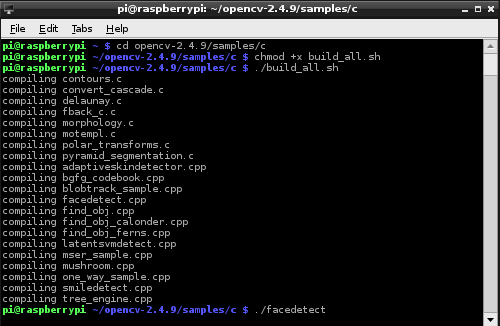
\includegraphics[scale=0.5]{Figs/Lena02.png}}
\subfigure[]{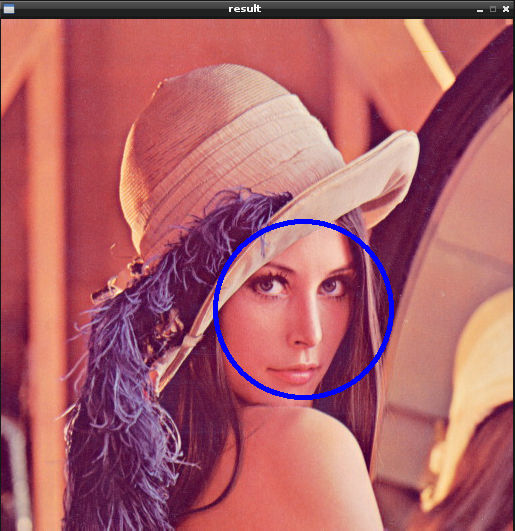
\includegraphics[scale=0.3]{Figs/Lena03.png}}
\subfigure[]{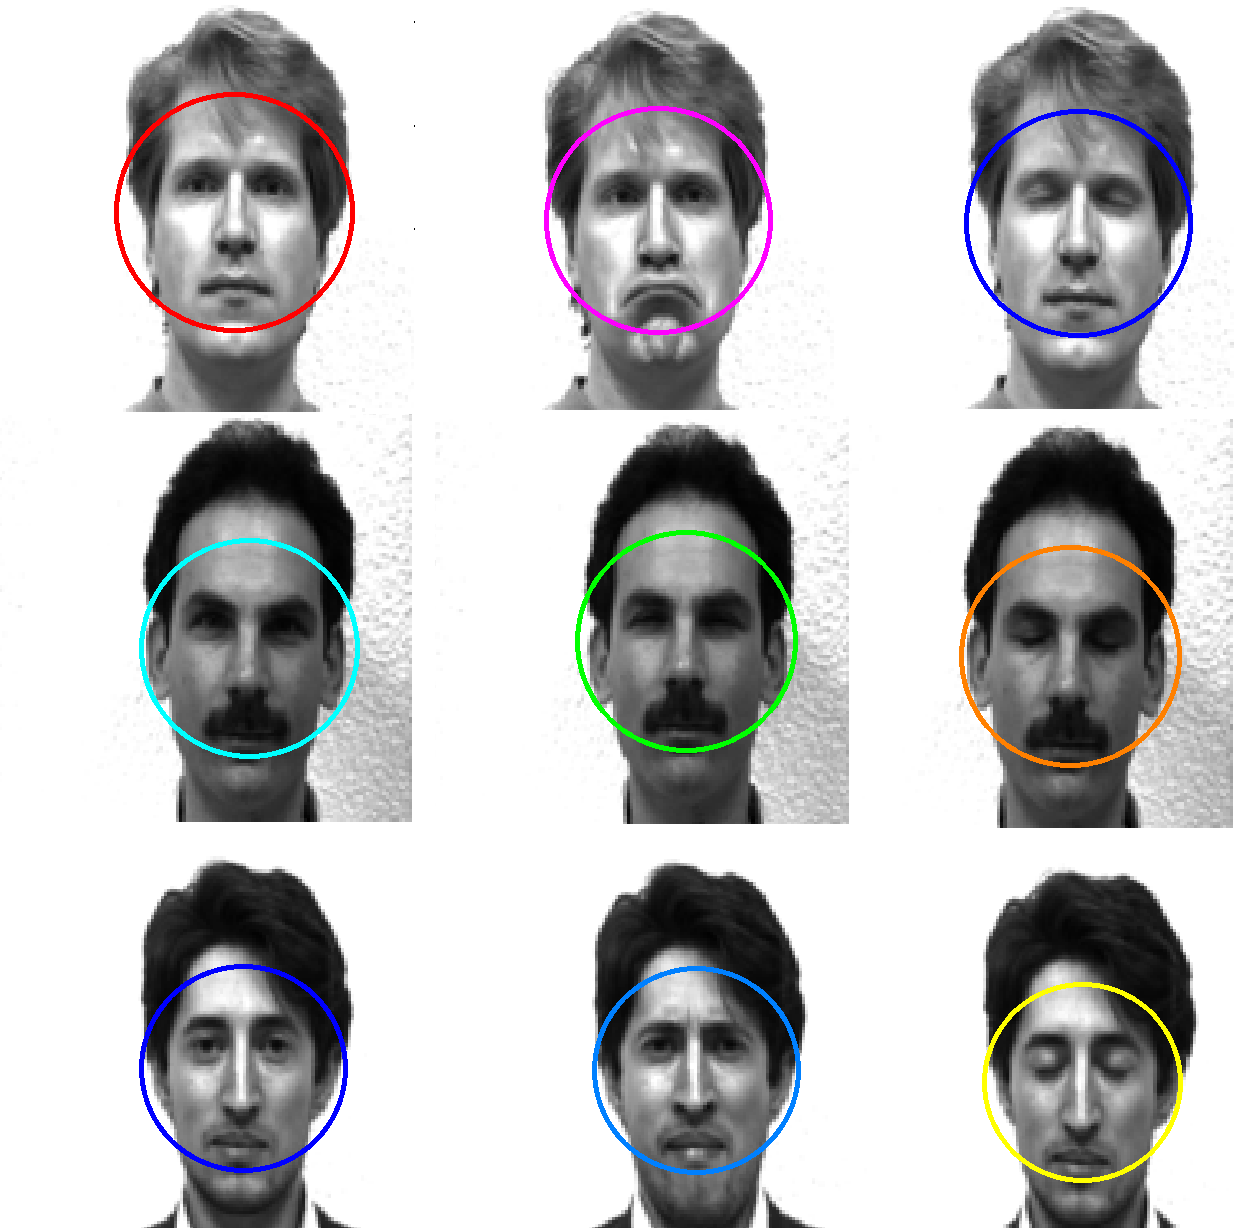
\includegraphics[scale=0.2]{Figs/result_screenshot_04.png}}
\caption{Segmentación de rostros utilizando los ejemplos de la librería OpenCV}
\label{Fig:EOp}
\end{figure}








%Para las tablas, el tratamiento es el mismo, salvo que el título debe ir ubicado en la parte superior de la tabla, como se muesta en la Tabla \ref{Tb:MSESimulatedAmber}. Acá se puede visualizar el MSE medio por pixel con respecto a la imagen original de las imagenes corruptas y corregidas. Resulta interesante que al aplicar distintos niveles de nouniformidad (lo que aleja a la imagen de la original en forma gradual), el resultado a la salida arroja un MSE practicamente unificado muy cercano a 0.05.
%\begin{table}[b]
% \centering
%\caption{MSE calculado al corregir ruido aditivo simulado para la cámara AMBER, \cite{GodoyNUC}.}
%\label{Tb:MSESimulatedAmber}
%\begin{tabular}{|c|c|c|}
% \hline
% \% & \textbf{MSE Imagen Corrupta} & \textbf{MSE Imagen Corregida} \\\hline
% 10	& 0.3876 & 0.0516 \\\hline
% 100  & 0.5022 & 0.0583 \\\hline
%\end{tabular}
%\end{table}

%Tanto las tablas como las imágenes, deben tener numeración propia, permitiendo así una mejor comprensión del texto y agregando cierta fluidez en la lectura pues permite seguir facilmente las referencias que Ud. realiza a ellas. Ambas se ubican solamente en la parte superior o inferior de una página o en una sola página pero nunca como flotantes en el texto. Se vuelve a recalcar que si una imagen o tabla es incluida, se debe al menos realizar una referencia a ella.

%Con respecto a las ecuaciones que Ud. deba utilizar, deben ir centradas, con numeración independiente ubicado a la derecha de la ecuación y entre paréntesis (si la ecuación es importante) y debe tener un pequeño análisis puntual o una breve explicación, como es el caso de la Ecuación~(\ref{Eq:Dmin}) que muestra la mínima dimensión de los quantum-dots formados en una heterojuntura del tipo-I con un potencial de confinamiento de $\Delta E_{c}$\footnote{Nótese porfavor que si la ecuación no relevante se recomienda incluirla en linea con el texto.}.
%\begin{equation}
% D_{min} = \frac{\pi \hslash}{\sqrt{2  m^{*}_{e}  \Delta E_{c}}}
%\label{Eq:Dmin}
%\end{equation}
%donde $m^{*}_{e}$ es la masa efectiva del electrón, \cite{KrishnaQD}.


% ***********************************************************************************
% ***********************************************************************************
% ***********************************************************************************
\newpage
\section{Conclusiones y trabajo futuro.}
\subsection{Conclusiones.}
\begin{itemize}\compresslist
\item El proyecto desarrollado analiza y describe lo que otros autores han realizado hasta el momento, las técnicas y algoritmos que existen para la detección de rostros.
\item Se acotó los algoritmos a utilizar en la memoria de título, los cuales serán: distancia Euclidiana, Eigenface y Support vector machine.
\item Se a escogido apoyarse en las librerías OpenCV para el desarrollo de este proyecto, a pesar de que en un principio se pensó en trabajar en Matlab debido a las facilidades de implementación y a la conexión disponible con la Raspberry Pi. Sin lugar a dudar OpenCV es más sólido y tiene bastantes códigos de guía.
\item El reconocimiento facial es un tema muy estudiado y de grandes aplicaciones requeridas en tiempos actuales. Si esto se le mezcla con un sistema embebido de código abierto y bajo costo puede llegar a ser una gran innovación.
\item Si es posible dar una solución a este problema, el tema ahora pasa ser eficientes y precisos en la implementación de la solución. Por eso la importancia a la que pueden llegar a ser las curvas de desempeño.

\end{itemize}
% ***********************************************************************************
% ***********************************************************************************

%Aquí se enumeran las conclusiones más importantes de lo realizado. Por ejemplo, indicar
%que se aumentó la eficiencia en un 2\%, es una conclusión. 
%Nunca concluir algo que no sea resultado o producto del trabajo realizado.
%Tenga cuidado con las palabras ``óptimo'', ``imposible'', ``obvio'', etc. Si utiliza
%el término ``óptimo'' es porque se optimizó algo y por tanto en el documento debiera
%existir un funcional que se maximizó o minimizó; la palabra ``imposible'' depende del
%momento histórico en que está la tecnología y el término ``obvio'' puede ofender a alguien,
%en particular a quienes no les resulte obvio.

% ***********************************************************************************
% ***********************************************************************************
\subsection{Trabajo futuro.}

Lamentablemente quedaron varios temas pendientes a desarrollar. En general son temas ligados a la programación.
\begin{itemize}\compresslist
\item Primero es terminar de implementar OpenCV en la Raspberry Pi a pesar de los errores de compilación.
\item Terminar la implementar el algoritmo de Mahalanobis, queda como tarea pendiente pensando como posible nuevo algoritmo a caracterizar.
\item Mejorar y estudiar en más profundidad en la segmentación de rostros.
\item Implementar SVM en la Raspberry Pi.
\item Crear la base de datos definitiva con la cual se trabajará el resto del proyecto.
\item Crear una batería de pruebas para poder caracterizar bajo distintas condiciones y obtener curvas de desempeño.
\end{itemize} 

%La idea es describir brevemente lo que se realizará en la Memoria de Título.
%Mientras más detallado sea lo expuesto, implica un trabajo más comprometido e
%interiorizado en el tema, lo que le gusta mucho a la comisión evaluadora.


% ***********************************************************************************
% ---------------------            BIBLIOGRAFIA                 ---------------------
% ***********************************************************************************
% LAS CITACIONES A DOCUMENTOS O ARTICULOS, SE DEBE HACER CONFORME AL FORMATO
% DADO POR LA IEEE. SE ADJUNTA PDF
% Ref: http://www.ieee.org/portal/cms_docs_iportals/iportals/publications/pubservices/confpub/ieeecitationref.pdf


\begin{thebibliography}{}
\addcontentsline{toc}{section}{Bibliografía}

\bibitem{UCarlosIII} Edwin Arturo Vega Aquino,``Detección y seguimiento de rostros'', Informe proyecto de fin de carrera, Universidad Carlos III de Madrid, 2011.
\bibitem{ElectronicoUdeC}``Reconocimiento de rostros evaluación de la aplicación de tres algoritmos al reconociemiento facial'', informe de memoria de título de Ingeniería Civil Electrónica, Depto. Ing. Eléctrica, Universidad de Concepción, 2001. 
\bibitem{VniversitatDValencia} Marcelo J. Armengot Iborra, ``Análisis comparativo de métodos basados en subespacios aplicados al reconocimiento de caras'', Vniversitat De València, 2006.
\bibitem{Bovik} Alan C. Bovik, \textit{`` The Essential Guide to Image Processing''},Academic Press, 2009 , Capítulo 24, pp. 667-713.
\bibitem{Paper01} R. Chellappa, C. L. Wilson, and S. Sirohey. `` Human and machine recognition of faces: a survey''. Proc. IEEE, 83:705–740, 1995.
\bibitem{JPhillips}P. J. Phillips, H. Moon, S. Rizvi, and P. J. Rauss. The FERET evaluation methodology for facerecognition algorithms.IEEE Trans. Pattern Anal. Mach. Intell.,22:1090–1104, 2000.
\bibitem{Libro02} Jian Guo Liu, Philippa Mason,``\textit{Essential Image Processing and GIS for Remote Sensing}'' ,John Wiley \& Sons, 2013, Capítulo 8, pp. 91-102.
\bibitem{Turk} M. Turk and A. Pentland. ``Eigenfaces for recognition'' .J. Cogn. Neurosci., 3:72–86, 1991.
\bibitem{RaspberryTollSyst} Md. Kawser Jahan Raihan  \textit{et al.}. ``Raspberry Pi Image Processing Based Economical Automated Toll System''.
Global Journal of Researches in Engineering Electrical and Electronics Engineering  \textbf{13} (2013) 34-41.
\bibitem{Viola} Paul Viola and Michael J. Jones
`` Robust Real-Time Face Detection''.,International Journal of Computer Vision \textbf{57(2)}, (2004) 137–154. 
\bibitem{ActasTdeI}
Josep Arnal García, Sergio Cuenca Asensi, Higinio Mora Mora, Francisco Moreno Seco (2010). \textit{Actas del $1^{er}$ Workshop en Tecnologías de la Informática} [Online].
Available url: \url{http://www.iuii.ua.es/master_ti/actas2010.pdf}\\
File: actas2010.pdf

\bibitem{TrabajoRaspiUdeC}
Víctor Garcés, Pablo Gleisner. \textit{``Sistemas de visión en dispositivos embebidos sobre linux"}, Univ. de Concepción, Concepción, Chile, 2013. 

\bibitem{Medina} Mario Medina C. Sistemas (2015). \textit{Introducción a Sistemas Computacionales} [Online].
Avaible url: \url{http://mondrian.die.udec.cl/~mmedina/Clases/SisComp/2014-2/SisComp-01-Intro.pdf}\\
File: SisComp-01-Intro.pdf
\bibitem{yaleface} Página Web de Yale Face Database url{http://vision.ucsd.edu/content/yale-face-database}.
\bibitem{Sirovich} L. Sirovich and M. Kirby  ``Low-dimensional procedure for the characterizacion of human faces'', Journal of the Optical Society of America A, 4(3): 519-524,1987.

\bibitem{EigenfaceEspa}  Franco Chichizola, Armando De Giusti, and Marcelo Naiouf. ``Eigenfaces de Imagen Reducida para el Reconocimiento Automático de Rostros''. RedUNCI, pag. 812-823, 2003.
\bibitem{bunschoten} Tijmen Majoor (2000). ``Face detection using color based region of interest selection''[Online].Avaible url:\\
 \url{http://www.science.uva.nl/research/ias/masterProjects/MajoorThesis.pdf} \\
 File: MajoorThesis.pdf
\bibitem{PaginaRPI} Raspberry Pi(2015). \textit{¿Qué es una Raspberry Pi?} Avaible url:   \url{https://www.raspberrypi.org/help/what-is-a-raspberry-pi/}
\bibitem{RoboPapa} RoboPapa (2014). \textit{Install Open CV on Raspberry Pi}[Online]\\
Avaible url: \url{http://www.robopapa.com/Projects/InstallOpenCVOnRaspberryPi}

\bibitem{AmirFa} Amir Faizi. ``Robust Face Detection Using Template Matching Algorithm", Thesis for the degree of Masters of Applied Science, Dep. of Electrical Engineering, University of Toronto, 2008.

\bibitem{SebastianGodoy} S. E. Godoy. ``Introduction to Support Vector Machines (SVM) Classifier''. Application to MS data, ECE - CHTM
University of New Mexico Albuquerque, NM, USA, 22 July, 2011.

\bibitem{HardwarePiPeri} Xataka(2015) \textit{Raspberry Pi 2 Model B: más potente y con soporte Windows 10} Avaible url: \url{http://www.mamaluchona.com/sistemas-it/raspberry-pi-pi-pi-pi-pi-en-palabras-sencillas/}

\bibitem{ImagenesPiCam} Bricogeek(2015) \textit{Cámara de 5MP para Raspberry Pi}, Avaible url: \url{http://tienda.bricogeek.com/raspberry-pi/569-camara-de-5mp-para-raspberry-pi.html}
\bibitem{Datasheet} Especificaciones técnicas Raspberry Pi(2014), Avaible url:\url{http://www.element14.com/community/servlet/JiveServlet/previewBody/68376-102-1-295702/RPI-BPLUS-V1_2-SCHEMATIC-REDUCED.pdf}

% Acá comienzan los ítemes
%\bibitem{ReevesMT}
%Rodrigo A. Reeves,
%``Compensación de Ruido Espacial en Sistemas de Imágenes con Sensores Infrarrojos'',
%Informe de Memoria de Título de Ingeniería Civil Electrónica, Depto. Ing. Eléctrica, Universidad de Concepción,
%Chile, 2002.


%
%\bibitem{TorresMSc}
%Flavio Torres Vicencio,
%``Corrección de no-uniformidad de imágenes infrarrojas usando un filtro adaptivo con el algoritmo RLS'',
%Tesis M.S.,  Depto. Ing. Eléctrica, Universidad de Concepción, Chile, 2005.
%
%\bibitem{TorresPhD}
%Sergio Torres Inostroza,
%``A Kalman-Filtering Approach for Non-Uniformity Correction in Infrared Focal-Plane Array Sensors'',
%Disertación Ph.D., Dept. of Electrical Engineering, Univ. of Dayton, Ohio, USA, 2001.
%
%\bibitem{GodoyNUC}
%S. E. Godoy, S. N. Torres, J. E. Pezoa, M.M. Hayat, and Q. Wang. ``Nonuniformity Correction Algorithm Based on a Noise-Cancellation System for Infrared Focal-Plane Arrays''. Accepted in the SPIE Defense and Security Symposium, to be held at Orlando, FL, USA, 9-13 April, 2007.
%
%\bibitem{KrishnaQD}
%Sanjay Krishna. ``Quantum Dots-in-a-well Infrared Photodetectors''. Journal of Physics D: Appl. Phys. \textbf{38} (2005) 2142-2150.



%\bibitem{fibics}
%Página web de Fibics Inc. \verb|http://www.fibics.com|.

\end{thebibliography}

% Contenido del documento
\newpage
\appendix
\section{Apéndices}
\subsection{ Raspberry Pi y Cámara}
\begin{figure}[H]
\centering
\subfigure[]{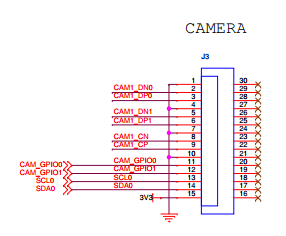
\includegraphics[scale=0.8]{Figs/DataSheet1.png}}
\subfigure[]{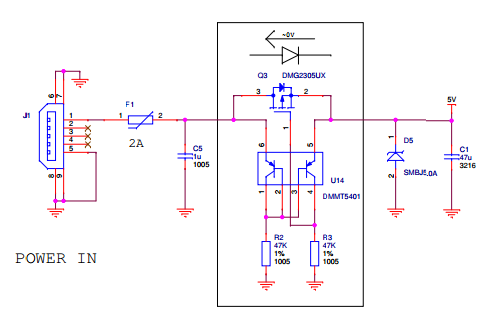
\includegraphics[scale=0.8]{Figs/DataSheet2.png}}
\subfigure[]{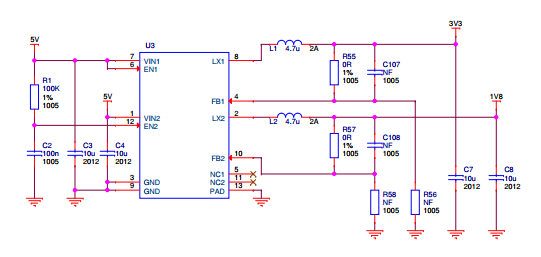
\includegraphics[scale=0.8]{Figs/DataSheet3.png}}
\caption{a)DataSheet Raspberry Pi Cam b) c)Esquema reducido de Raspberry Pi modelo B+ v1.2, \cite{Datasheet}}
\label{Fig:Datasheet}
\end{figure}
\end{document}